\chapter{Kajian Pustaka}
Pada bab ini disajikan penjelasan sejumlah teori, konsep dan gagasan terkait dengan domain penelitian pengenalan emosi manusia. Diawali dengan penjelasan lebih lengkap atas latar belakang yang disarikan dari sumber-sumber multidisiplin yang relevan dari bidang psikologi, sosial, biologi, statistika, dan lain-lain. Dilanjutkan dengan pemaparan penelitian-penelitian terkait meliputi alur berpikir dalam penentuan berbagai pendekatan yang diusulkan serta set data publik yang digunakan pada penelitian ini, perbandingan pendekatan serta hasil eksperimen dari sejumlah penelitian terkait mutakhir dan sedikit mengenai teknik-teknik yang diadopsi pada penelitian ini. Kemudian dipaparkan beberapa metode, teknik dan formula yang disoroti pada penelitian ini meliputi filter Gabor, filter Log-Gabor, \acrshort{gcns} dan \acrshort{frs}. Diakhiri dengan deskripsi singkat mengenai beberapa pustaka utama yang dipakai dalam pelaksanaan eksperimen.

\section{Pengenalan Emosi}
Emosi merupakan bagian dari komunikasi. Komunikasi berperan penting dalam interaksi sosial di beragam sistem sosial. Studi komunikasi merupakan studi multidisipliner yang melibatkan psikologi, sosiologi, antropologi dan linguistik \shortcite{mandal2014understanding}. Pada teknologi informasi, komunikasi spesifik dipelajari dalam interaksi manusia dan komputer \shortcite{cowie2001emotion,fragopanagos2005emotion}.

Komunikasi adalah untuk berbagi realitas bersama \shortcite{cobley2008communication}. Membaca pikiran orang lain ---atau membuat kesimpulan tentang keadaan pikiran orang lain--- dalam komunikasi penting dilakukan dalam bertindak kooperatif. Ada banyak cara untuk setiap orang menyampaikan suatu makna. Sementara itu, sebuah kalimat dapat memiliki makna yang berbeda dalam konteks yang lain \shortcite{miller1999knowing}. Selain kemampuan memahami konteks, penting untuk seseorang memiliki kemampuan mengetahui sifat dan latar belakang dari lawan bicara mereka dalam komunikasi. Sebab apa yang orang sampaikan mungkin berbeda dari apa yang mereka pikirkan. Lingkungan juga berkontribusi dalam mempengaruhi bagaimana orang berpikir \shortcite{entman1989media}.

Membaca pikiran yang tidak akurat dapat berdampak pada kebingungan, kesalahpahaman hingga berujung kepada konflik hidup dan mati. Penipuan adalah salah satu dampaknya, sehingga pengenalan tanda-tanda kebohongan menjadi masalah yang menantang \shortcite{ekman2009telling,vrij2019reading}. Masalah komunikasi ini menjadi semakin rumit dalam komunikasi antar kultur. Di mana kompleksitas dan keanekaragaman dialek yang dimiliki oleh masing-masing bahasa menyulitkan dalam proses interpretasi dan penerjemahan ke dalam bahasa lain \shortcite{purnell2018cross}.

Komunikasi terbagi menjadi tiga model (Gambar \ref{fig:tipekomunikasi}), yaitu berdasarkan metode atau media, arus informasi dan hubungan organisasi. Model kedua dan ketiga mengacu pada komunikasi di lingkungan organisasi fungsional \shortcite{postmes2001communication,elving2005role,lunenburg2010formal,kandlousi2010organizational}. Sedangkan model pertama lebih generik, mengacu pada komunikasi perseorangan di mana faktor emosi menjadi lebih diperhatikan.
\begin{figure}[ht]
    \centering
    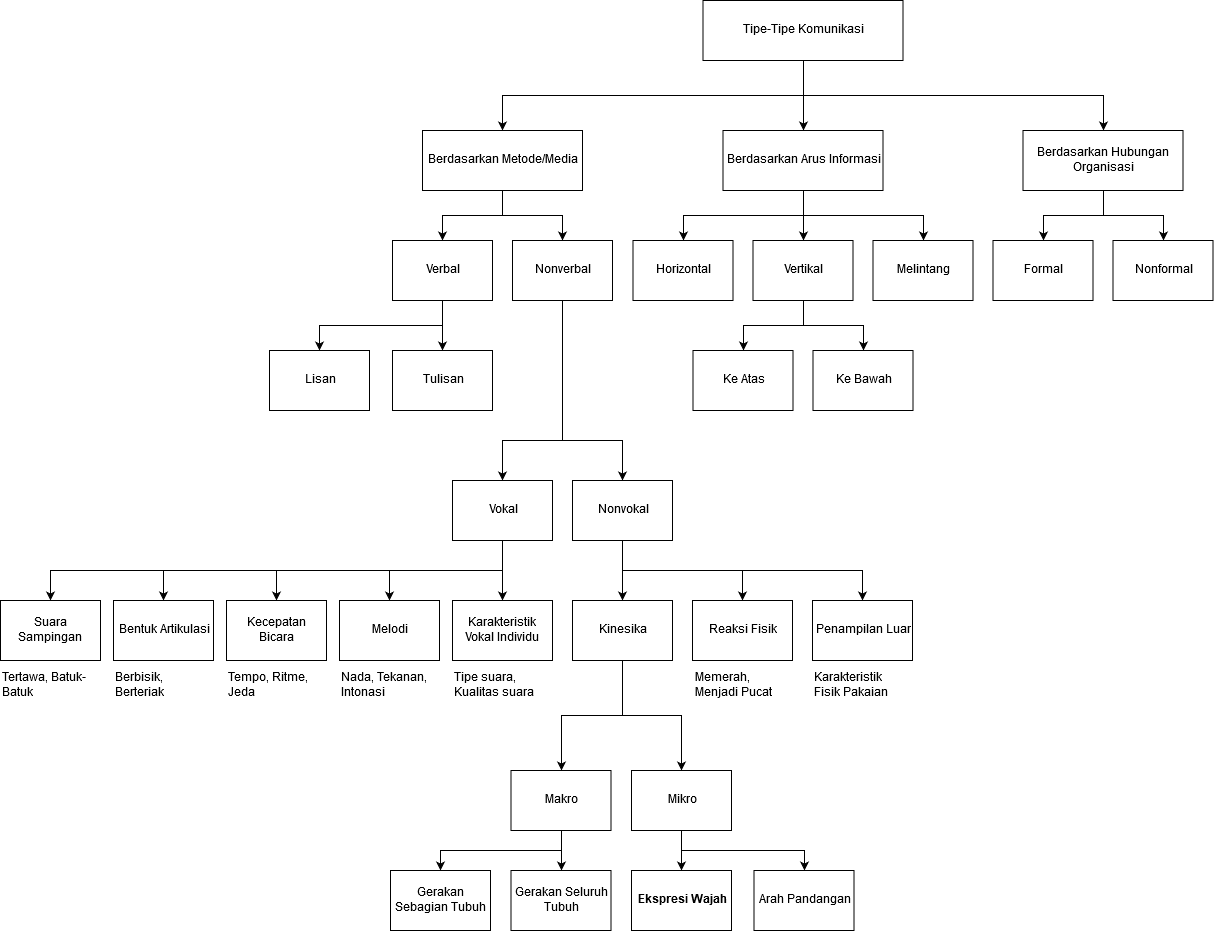
\includegraphics[width=14cm]{gambar/tipe_tipe_komunikasi.png}
    \caption[Pembagian Model-Model Komunikasi]{Pembagian Model-Model Komunikasi (\protect\shortciteNP{surkamp2014non};\\www.businesscommunicationarticles.com)}
    \label{fig:tipekomunikasi}
\end{figure}

Antara emosi, \textit{mood} dan perasaan, memiliki definisi yang berbeda di kalangan para ahli. Beberapa di antara mereka membedakannya. Dalam membandingkan emosi dan \textit{mood}, \shortciteA{ekman1994nature} menyatakan bahwa 1) \textit{mood} berlangsung lebih lama, 2) \textit{mood} lebih mudah terprovokasi, 3) \textit{mood} lebih sulit untuk dimodulasi, 4) \textit{mood} tidak memiliki ekspresi wajah unik sendiri, dan 5) \textit{mood} lebih sulit disadari penyebabnya dibandingkan dengan emosi.

Dalam kaitan emosi dengan perasaan/sentimen, \shortciteA{freedman2017emotions} menyatakan bahwa perasaan merupakan campuran dari emosi dan bertahan lebih lama. Perasaan muncul ketika membiarkan emosi, yang biasanya hanya bertahan selama enam detik. Menurut \shortciteA{perez2018emotions}, sentimen akan tetap bertahan selama disadari dan dipikirkan. Berbeda dengan emosi, sentimen dikendalikan secara sadar oleh pikiran. Sementara sebagian ahli membedakan perasaan dengan sentimen \shortcite{munezero2014they}. Meskipun konvensi dalam masalah ini belum terjadi, mereka bersepakat bahwa emosi bertahan dalam rentang waktu relatif lebih pendek.

Emosi merupakan sesuatu yang amat kompleks untuk dipahami bahkan secara mendalam. Emosi seseorang terbentuk atas berbagai faktor, seperti kepribadian \shortcite{arnold1960emotion}, bahasa \shortcite{lutz1990language}, kemampuan adaptasi \shortcite{smith1990emotion}, kultur \shortcite{kitayama1994emotion}, kondisi kesehatan \shortcite{pennebaker1995emotion}, kemampuan pengambilan keputusan \shortcite{schwarz2000emotion}, harapan \shortcite{kenny2003action}, motivasi \shortcite{bradley2007emotion} dan lain-lain. Seseorang dapat memahami signifikansi dan nilai dari sebuah emosi jika dia pernah mengalaminya sendiri \shortcite{mun2019knowing}.

Emosi merupakan sesuatu yang abstrak bagi orang lain. Akan tetapi, pada umumnya, emosi memiliki bentukan yang dapat diamati. Secara alami, emosi membentuk perilaku temporal seseorang \shortcite{baumeister2007emotion}. Bentukan tersebut hanya diakui akurat jika hal itu bersifat evaluatif \shortcite{mun2019knowing}.

Pengenalan emosi dapat dilakukan dengan berbagai teknik seperti melalui pengenalan ekspresi wajah \shortcite{canedo2019facial}, ucapan \shortcite{khalil2019speech}, tulisan \shortcite{seyeditabari2018emotion} atau sinyal-sinyal lain \shortcite{wagh2019electroencephalograph}. Masing-masing pendekatan tersebut dianggap representatif dalam pemodelan pengenalan emosi yang presisi dan akurat.

Pengenalan emosi melalui ekspresi wajah sendiri belum mampu mencerminkan emosi secara tepat dan utuh \shortcite{fernandez2013emotion}. Namun sejauh ini, pengenalan emosi melalui ekspresi wajah dinilai paling akurat. Sebab sebagian besar komunikasi adalah bersifat nonverbal \shortcite{lapakko2007communication,mehrabian1967decoding,mehrabian1967inference}.

\begin{figure}[t]
    \centering
    \begin{subfigure}[t]{6cm}
        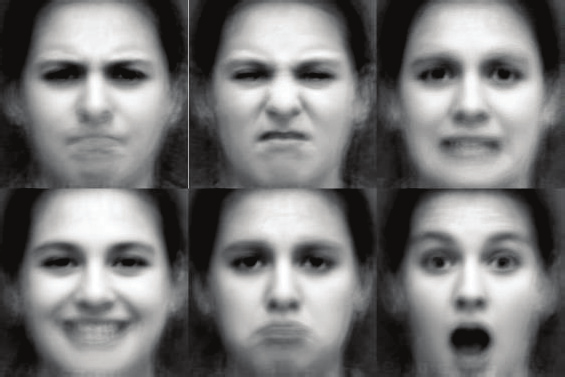
\includegraphics[width=6cm]{gambar/rerata_ekspresi_wajah_barat.png}
        \caption{}
    \end{subfigure}
    ~~~
    \begin{subfigure}[t]{6cm}
        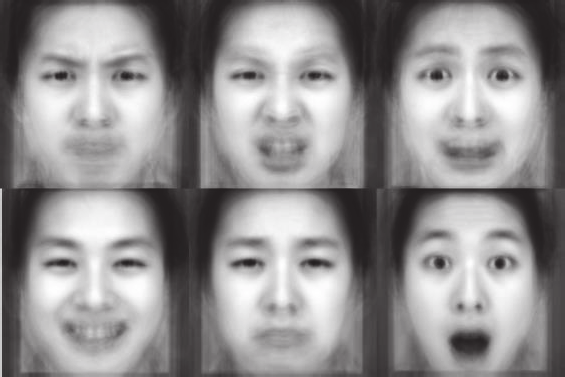
\includegraphics[width=6cm]{gambar/rerata_ekspresi_wajah_asia.png}
        \caption{}
    \end{subfigure}
    \caption[Perbedaan Rerata Pola Ekspresi Wajah Orang (a) Barat dan (b) Asia dalam Enam Kelas Emosi Berbeda]{Perbedaan Rerata Pola Ekspresi Wajah Orang (a) Barat dan (b) Asia dalam Enam Kelas Emosi Berbeda \protect\shortcite{benitez2017analysis}}
    \label{fig:rerataekspresiwajah}
\end{figure}

\begin{figure}[t]
    \centering
    \begin{subfigure}[t]{7.5cm}
        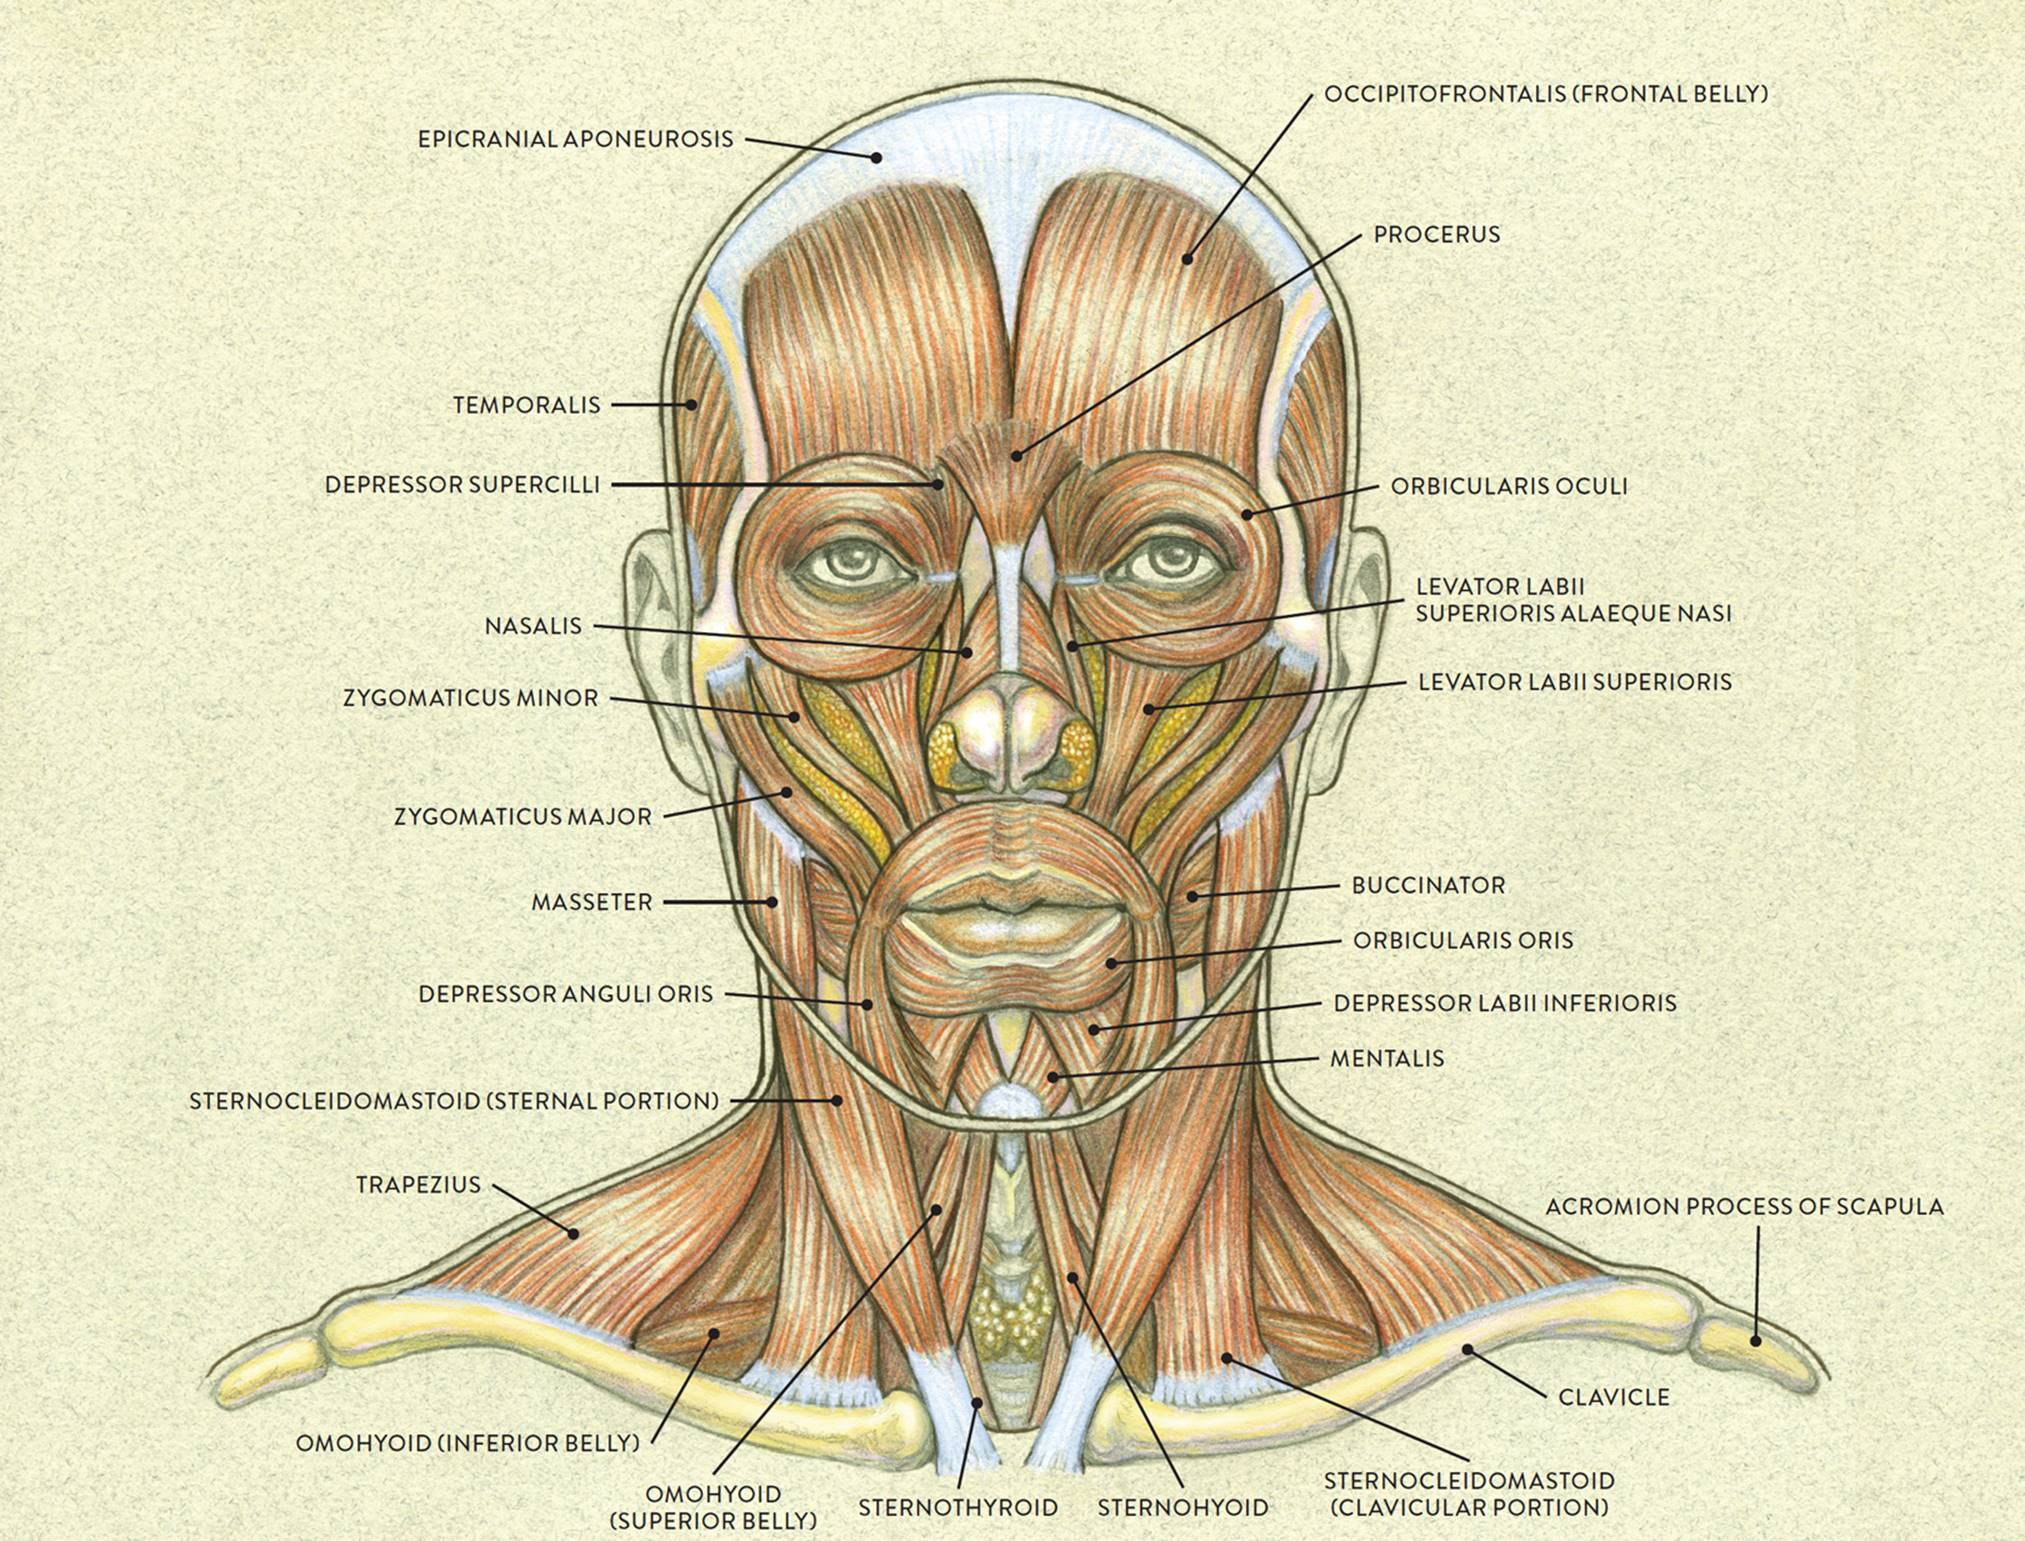
\includegraphics[width=7.5cm]{gambar/classic_human_anatomy_motion1.jpg}
    \end{subfigure}
    \begin{subfigure}[t]{4.5cm}
        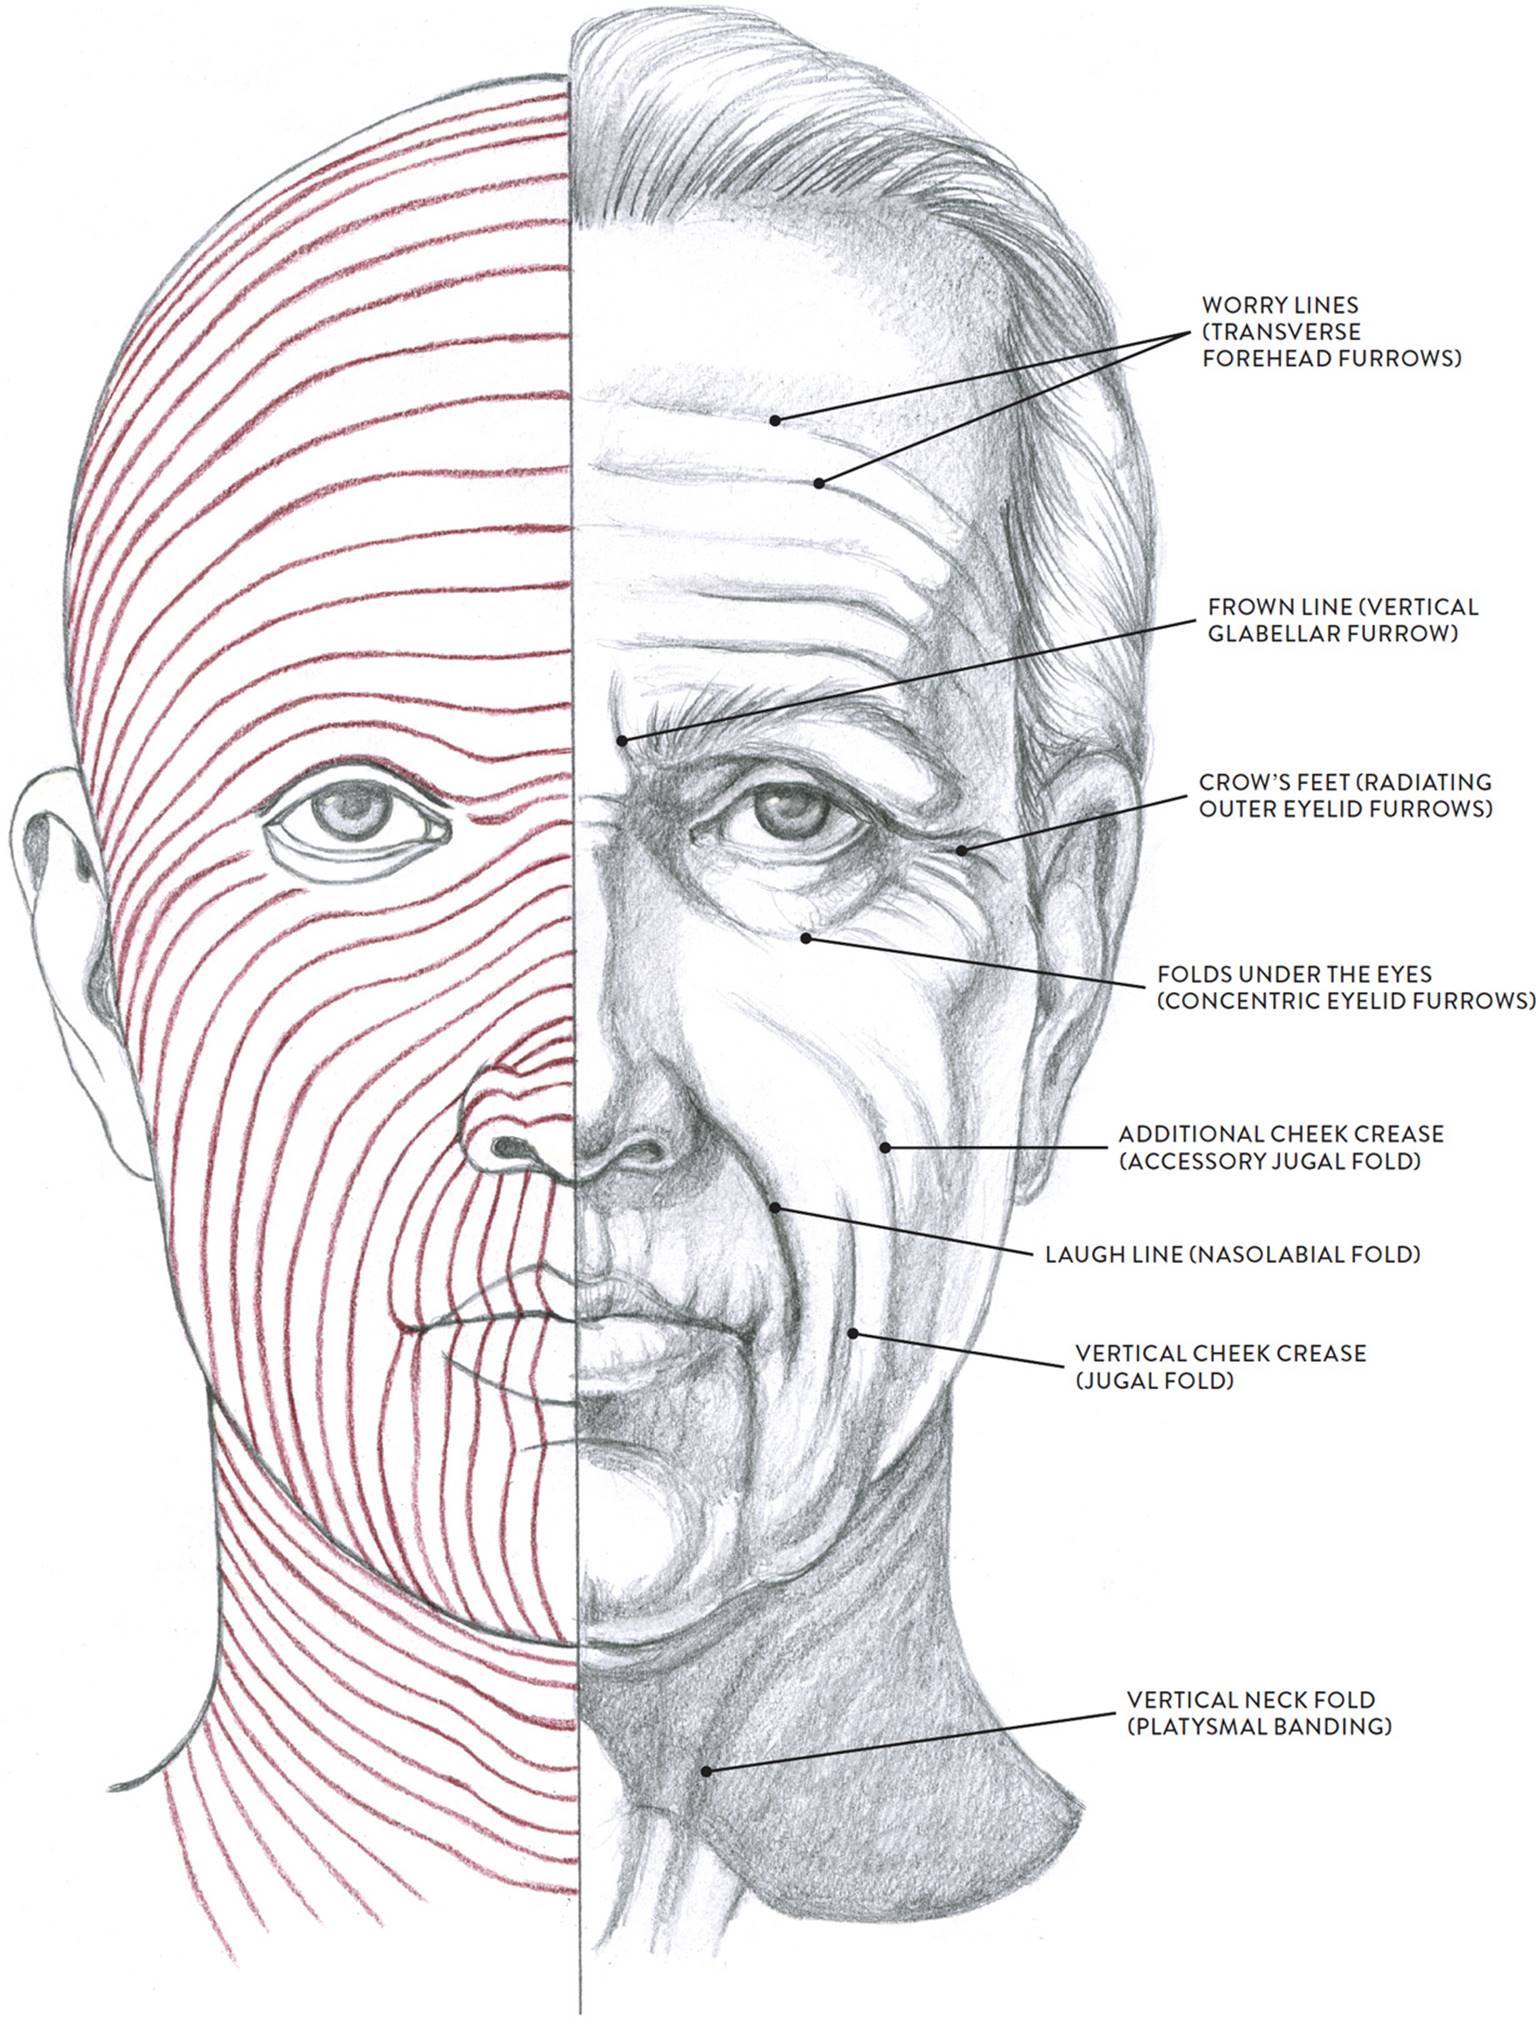
\includegraphics[width=4.5cm]{gambar/classic_human_anatomy_motion2.jpg}
    \end{subfigure}
    \caption[Otot-Otot Wajah Terkait Ekspresi Wajah]{Otot-Otot Wajah Terkait Ekspresi Wajah \protect\shortcite{winslow2015classic}}
    \label{fig:musclesface}
\end{figure}
Keuniversalan emosi masih terus diperdebatkan hingga sekarang ini \shortcite{gendron2014perceptions,hall2019nonverbal,jack2012facial}. \shortciteA{ekman1970universal} berpendapat bahwa sejumlah ekspresi wajah (\gls{sixbasicemotions}) bersifat universal, yaitu \textit{angry}, \textit{disgust}, \textit{fear}, \textit{happy}, \textit{sad}, \textit{surprise}, dan \textit{neutral}. Sebagian besar ilmuwan yang memenuhi kualifikasi \shortciteA{ekman2016scientists} menyetujui adanya bukti kuat pada keuniversalan emosi. Baru-baru ini terbukti bahwa \gls{sixbasicemotions} tidak berlaku antar kultur Asia dan Barat \shortcite{benitez2017analysis,benitez2018multicultural}. Gambar \ref{fig:rerataekspresiwajah} menunjukkan perbedaan yang cukup mendasar antara rerata pola ekspresi wajah dari kedua kultur tersebut.

Ekspresi wajah dapat dibedakan melalui lebih dari 10.000 kombinasi gerakan relatif lima belas otot bagian wajah (Gambar \ref{fig:musclesface}) \shortcite{ekman2004emotions,westbrook2019anatomy}. Kerutan kulit wajah karena usia, rona merah wajah, arah lirik dan kedipan mata serta ukuran pupil juga terlibat dalam pengenalan ekspresi wajah \shortcite{guo2013facial, kret2015emotional}.

\begin{figure}[t]
    \centering
    \begin{subfigure}[t]{6cm}
        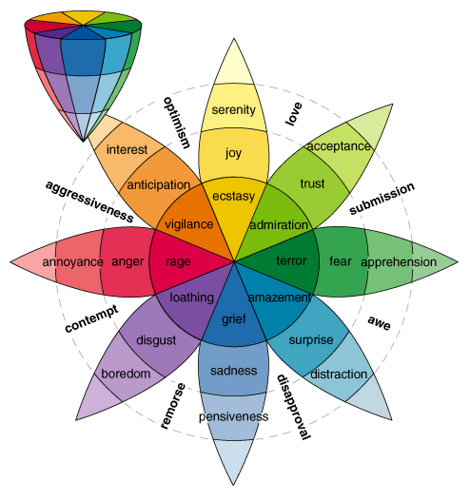
\includegraphics[width=6cm]{gambar/plutchik_wheel_emosi.jpg}
        \caption{\textit{Plutchik’s Wheel of Emotions} (https://www.theemotionmachine.com/\\classification-of-emotions/)}
        \label{fig:plutchikwheelemotions}
    \end{subfigure}
    \begin{subfigure}[t]{6cm}
        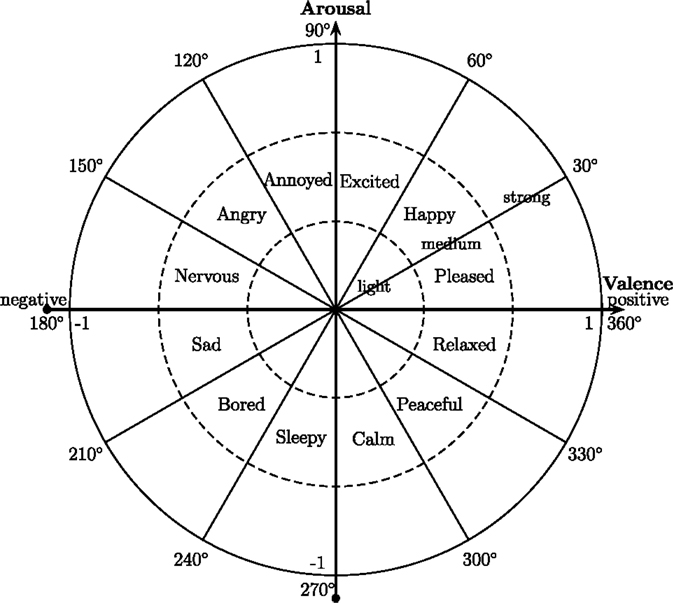
\includegraphics[width=6cm]{gambar/fuzzy_emosi.jpg}
        \caption{Lingkaran Emosi \textit{Fuzzy} \protect\shortcite{kowalczuk2016computational}}
        \label{fig:diagramemosifuzzy}
    \end{subfigure}
    \caption{Diagram Klasifikasi Emosi}
\end{figure}
Emosi tidak biner atau terdefinisi dengan baik, melainkan setiap emosi saling terhubung dan mempengaruhi satu sama lain menurut kedekatannya \shortcite{paiva2001safira}. Klasifikasi emosi tidak hanya terbatas pada model diskrit yang menghasilkan lima, enam atau 23 jenis emosi berbeda. Melalui pendekatan dimensional, \shortciteA{plutchik2013theories} memperkenalkan diagram emosi yang menghubungkan delapan jenis emosi dasar (Gambar \ref{fig:plutchikwheelemotions}). Melalui pendekatan \textit{fuzzy}, \shortciteA{kowalczuk2016computational} memperkenalkan lingkaran emosi dengan dua belas jenis emosi dasar (Gambar \ref{fig:diagramemosifuzzy}). Diagram pohon terstruktur \shortciteA{parrott2001emotions} bahkan mampu mendefinisikan hingga lebih dari seratus jenis emosi spesifik.

\newpage
\section{Penelitian Terkait}
\begin{figure}[t]
    \centering
    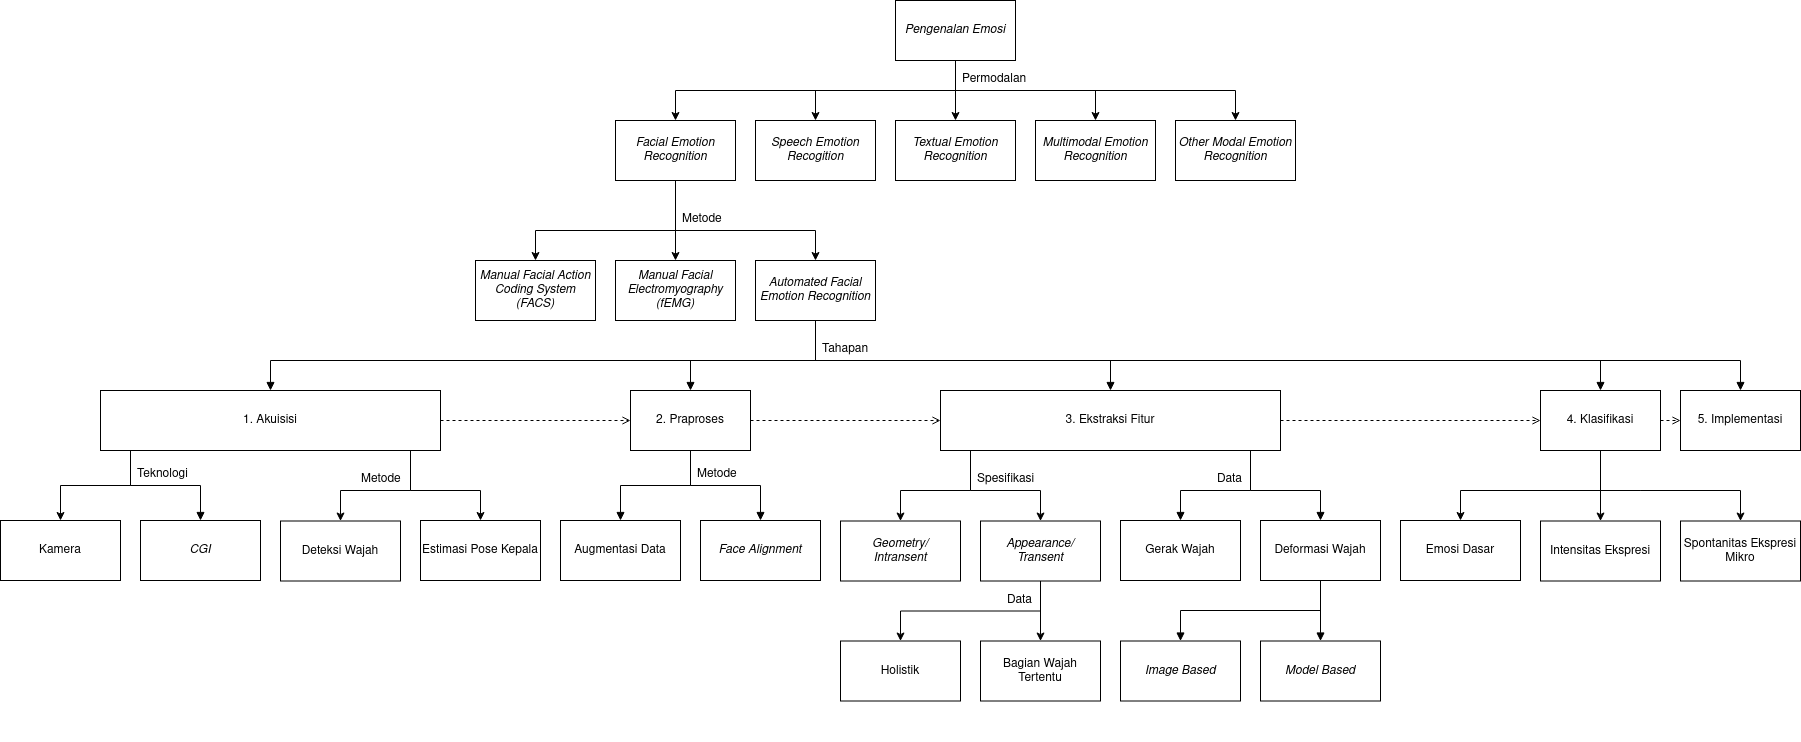
\includegraphics[width=14cm]{gambar/taksonomi_pengenalan_emosi.png}
    \caption[Taksonomi Pengenalan Emosi]{Taksonomi Pengenalan Emosi \protect\shortcite{sumathi2012automatic}}
    \label{fig:taksonomiemosi}
\end{figure}
Pengenalan emosi, terkait bidang ilmu komputer, memiliki domain penelitian yang sangat luas (Gambar \ref{fig:taksonomiemosi}). Berdasarkan jenis modal, pengenalan emosi dapat dilakukan baik melalui sinyal ucapan, tulisan, ekspresi wajah, sinyal digital ---seperti sinyal haptik dari \textit{drawing tablet} \shortcite{schrader2020linking}, sinyal aktifitas otak dari \textit{electroencephalogram} \shortcite{wagh2019electroencephalograph} dan sinyal tekanan dari \textit{keyboard} \shortcite{lv2008emotion}--- maupun kombinasi dari itu semua \shortcite{avots2019audiovisual,li2019fusion,mittal2019m3er}.

Pengenalan emosi melalui ucapan dapat dilakukan baik dengan pendekatan linguistik (tentang apa yang diucapkan) maupun paralinguistik (tentang bagaimana mengucapkannya) dalam komunikasi verbal. Dengan teknik-teknik pemrosesan sinyal, karakteristik unik tiap-tiap emosi dapat dikenali. Namun, belum ada konsensus mengenai set fitur standar untuk pengenalan ini. Sehingga menyulitkan pengevaluasian akurasi model pengenalan emosi dalam ucapan \shortcite{hook2019automatic,roy2020speech}. Bagaimanapun, hal ini merupakan tantangan terbesar bagi penelitian pengenalan emosi secara umum.

Pengenalan emosi melalui tulisan juga tergolong ke dalam kajian linguistik komputasi. Jika pengenalan emosi dalam ucapan cenderung meneliti mengenai gelombang bunyi dari wicara, maka pengenalan emosi dalam tulisan meneliti tentang tata bahasa yang terkandung dalam vektor-vektor kata baik dalam kumpulan frasa, kalimat maupun dokumen \shortcite{collobert2011natural,baali2019emotion}.

\begin{wrapfigure}{r}{4.6cm}
    \vspace{-0.5cm}
    \centering
    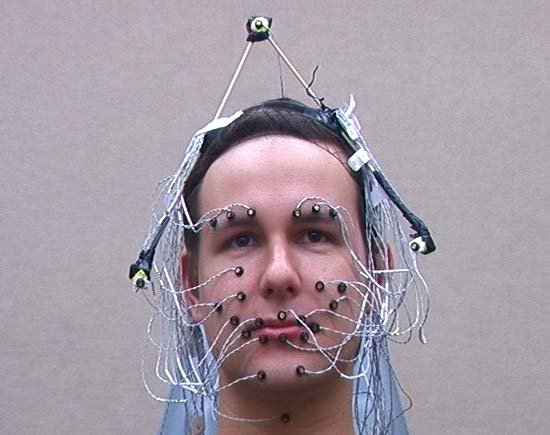
\includegraphics[width=4.5cm]{gambar/27_active_motion_capture_sensors.jpg}
    \caption[Contoh \textit{Facial Electromyography}]{Contoh \textit{Facial Electromyography} \protect\shortcite{gibert2010role}}
    \label{fig:contohfemg}
\end{wrapfigure}
Pengenalan emosi melalui ekspresi wajah menurut \shortciteA{wolf2015measuring} terbagi menjadi tiga metode, yaitu pelacakan aktivitas elektromiografi wajah, pengkodean aksi wajah dan rekognisi ekspresi wajah otomatis. Pelacakan aktivitas elektromiografi wajah atau \textit{facial electromyography} melibatkan penggunaan elektroda-elektroda yang dilekatkan pada permukaan wajah di titik-titik tertentu yang dianggap representatif (Gambar \ref{fig:contohfemg}). Sayangnya metode ini tidak dapat digunakan dalam situasi sosial sebab kompleksitas teknisnya. Namun, untuk mendeteksi aktivitas yang halus pada otot-otot wajah, metode ini sangat dapat diandalkan. Kesulitan yang dihadapi adalah menempatkan elektroda-elektroda tersebut pada posisi yang benar-benar tepat.

\begin{wrapfigure}{l}{4.7cm}
    \centering
    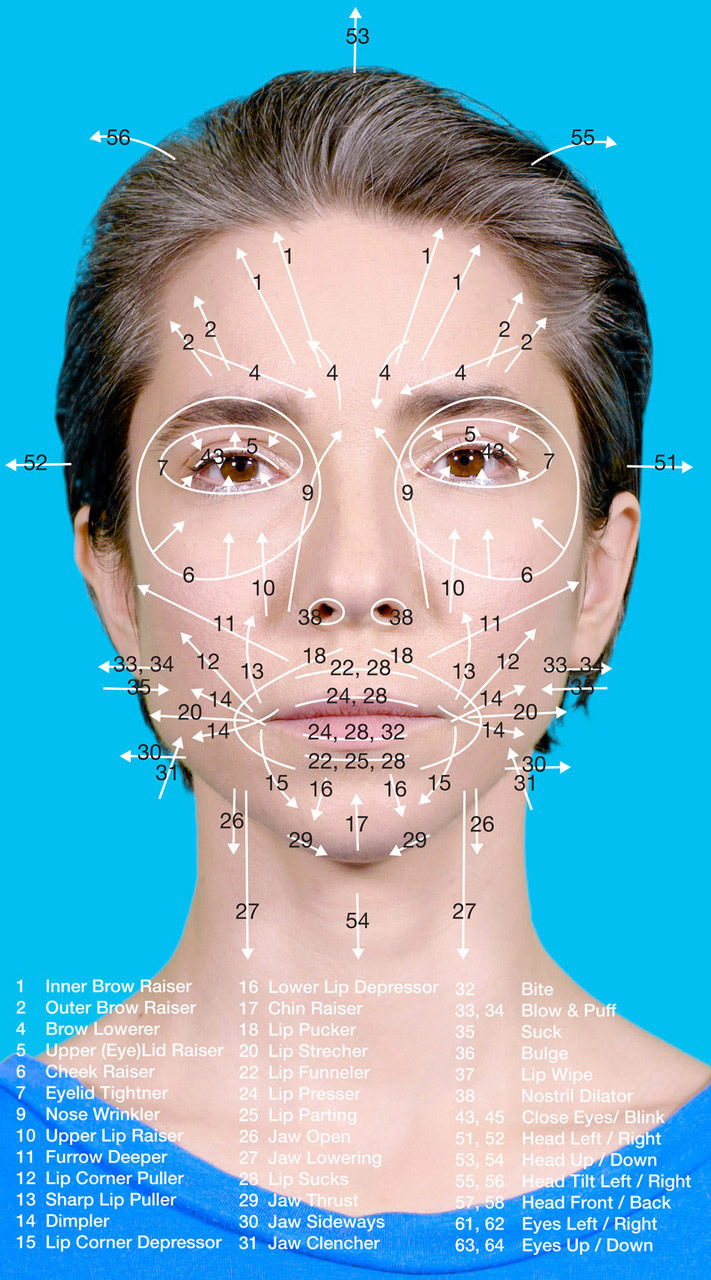
\includegraphics[width=4.7cm]{gambar/facs_coralie_vogelaar.jpg}
    \caption[Contoh \textit{Facial Action Units}]{Contoh \textit{Facial Action Units} (www.coralievogelaar.com)}
    \label{fig:contohfacs}
\end{wrapfigure}
Pengkodean aksi wajah atau \textit{facial action coding} \shortcite{ekman1997face} merupakan pengenalan emosi yang melibatkan analisis perubahan perilaku-perilaku otot-otot wajah yang kasat mata disebut sebagai unit aksi \textit{action units}. Unit-unit aksi ini didefinisikan secara manual, di antaranya adalah bagian kiri, kanan, luar dan dalam untuk tiap-tiap alis, mata, hidung, bibir dan mulut (Gambar \ref{fig:contohfacs}). Metode ini dapat meminimalkan bias oleh pengamat emosi. Namun proses analisis metode ini memerlukan bentukan emosi yang relatif kuat dan usaha manual yang banyak \shortcite{wolf2015measuring}. Dalam usaha meminimalkan waktu analisis pada perlakuan manual, pelacakan unit-unit aksi dikenali secara otomatis dengan pengukuran jarak relatif antar titik-titik wajah hasil deteksi tengara wajah atau \textit{facial landmarks} \shortcite{valstar2006fully}.

Pengenalan ekspresi wajah otomatis bekerja dengan cara menyandikan informasi ekspresi dari representasi wajah, baik informasi spasial dari tiap-tiap gambar statis maupun informasi hubungan temporal dari gambar-gambar sekuens, dengan bantuan \textit{machine learning}. Teknik \textit{machine learning} telah berkembang dari \textit{shallow learning} (di mana pemerolehan fitur-fitur wajah masih dilakukan secara manual) menjadi \textit{deep learning} (di mana pemerolehan fitur-fitur wajah diberikan seutuhnya kepada mesin). Teknik \textit{deep learning} telah terbukti jauh mengungguli metode-metode tradisional \shortcite{li2018deep}.

Pengenalan ekspresi wajah otomatis sangat bergantung pada kualitas dan kuantitas set data \textit{learning}\footnote{Penggunaan istilah set data \textit{learning} dalam konteks \textit{machine learning} mengacu kepada pengertian yang luas, yaitu mencakup set data \textit{training}, \textit{validation} dan \textit{test}.}. Maka dari itu, usaha memperoleh set data yang bagus menjadi tantangan tersendiri. Namun kekhawatiran pada pemerolehan set data ini tidak diperlukan lagi, sebab saat ini telah banyak orang dermawan yang bersusah payah untuk melakukannya. Set data tersebut sudah dilabeli dan disediakan gratis secara publik; penulis secara khusus bersyukur kepada para dermawan itu. Tinjauan mendetail mengenai beragam set data publik untuk pengenalan ekspresi wajah dapat ditemukan di \shortciteA{li2018deep}.

% TODO: bahas setiap komponen di taksonomi

\begin{figure}[t]
    \centering
    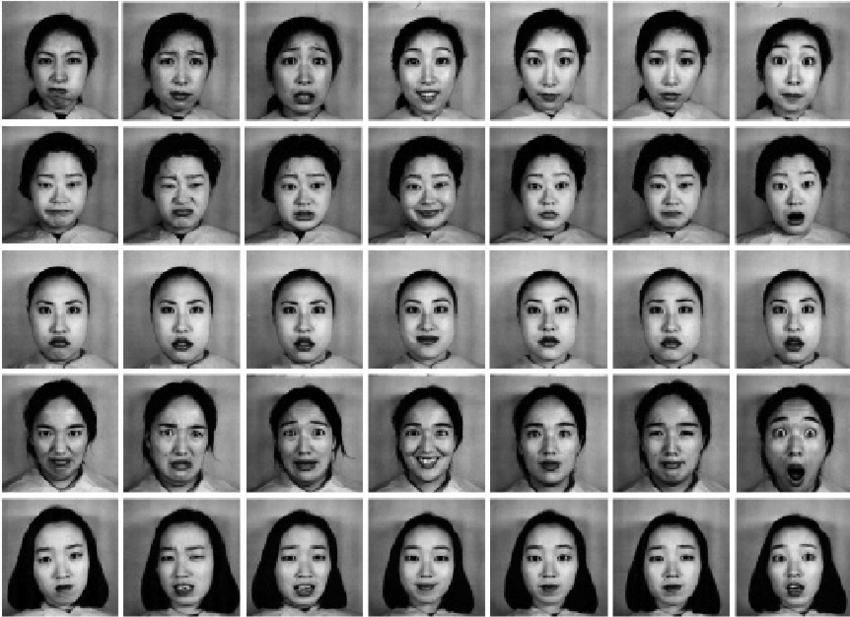
\includegraphics[width=14cm]{gambar/pratinjau_jaffe.jpg}
    \caption[Pratinjau Set Data JAFFE]{Pratinjau Set Data JAFFE \protect\shortcite{zhao2011facial}}
    \label{fig:pratinjaujaffe}
\end{figure}
Sebagian besar pengenalan ekspresi wajah otomatis memanfaatkan set data wajah frontal, contohnya JAFFE \shortcite{lyons1998coding}, CK+ \shortcite{lucey2010extended} dan EmotioNet \shortcite{fabian2016emotionet}. Gambar \ref{fig:pratinjaujaffe} memperlihatkan beberapa contoh gambar wajah frontal dari JAFFE. Mereka telah berhasil mencapai performa akurasi lebih dari 95\%. Model pengenalan ekspresi wajah melalui pendekatan teknik yang diusulkan oleh \shortciteA{zhou2019facial} bahkan mencapai akurasi sebesar 100\% untuk CK+. Namun, di samping kesulitan akuisisi data wajah frontal, model yang dikembangkan dengan set data wajah frontal menjadi tidak relevan pada penerapan di kondisi alam liar \shortcite{li2018deep}.

Pengenalan ekspresi wajah menggunakan set data wajah nonfrontal, contohnya FER-2013\footnote{Set data FER-2013 merupakan set data wajah nonfrontal publik yang paling populer digunakan dalam banyak penelitian pengenalan ekspresi wajah. Sejauh pengetahuan terbaik penulis, belum ada set data wajah nonfrontal lain yang tersedia secara publik.} \shortcite{goodfellow2013challenges}, hingga sekarang belum mencapai kepuasan berarti. Hasil survei penulis menuturkan bahwa akurasi tertinggi yang berhasil diraih saat ini untuk FER-2013 adalah 75,42\% \shortcite{georgescu2019local}. Untuk menemukan metode optimal yang mampu meningkatkan akurasi model pengenalan ekspresi wajah nonfrontal, maka penulis melakukan survei pada penelitian-penelitian terbaru. Penulis membatasi survei tersebut pada praproses, ekstraksi fitur dan model \acrshort{cnn} berikut performanya. Tabel \ref{tab:penelitiansota} memberikan gambaran mengenai hasil penerapan berbagai usulan metode penelitian dalam pengenalan emosi otomatis melalui ekspresi wajah.
\begin{table}[t]
    \caption{Penelitian Terkait}
    \label{tab:penelitiansota}
    \scriptsize
    \begin{tabular}{|C{1.4cm}|c|C{1.1cm}|C{2cm}|C{1.6cm}|C{1cm}|C{1cm}|c|}
        \hline
        \multicolumn{1}{|c|}{\multirow{2}{*}{Referensi}} & \multicolumn{1}{c|}{\multirow{2}{*}{Basis Data}} & \multicolumn{1}{C{1.1cm}|}{Tipe Jaringan} & \multicolumn{1}{C{2cm}|}{\multirow{2}{*}{Seleksi Data}} & \multicolumn{1}{c|}{\multirow{2}{*}{Praproses}} & \multicolumn{1}{C{1cm}|}{Ekstraksi Fitur} & \multicolumn{1}{c|}{\multirow{2}{*}{\textit{Classifier}}} & \multicolumn{1}{C{1cm}|}{Performa (\%)} \\
        \hline\hline
        \shortciteNP{georgescu2019local} & \multirow{15}{*}{\centering FER-2013} & \multirow{2}{*}{CNN, \textit{NE}} & \multirow{2}{*}{k-NN} & \multirow{4}{1.6cm}{\centering \textit{DA}} & \multirow{2}{1cm}{\centering CNNs + BOVW} & \multirow{2}{*}{\centering SVM} & \multirow{2}{*}{\centering 75,42} \\ % kutip FER+ jika diperlukan
        \cline{1-1}\cline{3-4}\cline{6-8}
        \shortciteNP{agrawal2020using} &  & \multirow{4}{*}{CNN} & \multirow{2}{2cm}{\centering 80\% set \textit{training}, 20\% set \textit{test}} &  & \multicolumn{2}{c|}{\multirow{2}{*}{CNN (16; 0,46M)$^\ast$}} & \multirow{2}{*}{65,23} \\
        \cline{1-1}\cline{4-8}
        \shortciteNP{engin2018face} &  &  & \multirow{11}{2cm}{\centering 28.709 set \textit{training}, 3.589 set \textit{validation}, 3.589 set \textit{test}} & \multirow{2}{*}{\textit{PN}} & \multicolumn{2}{c|}{\multirow{2}{*}{VGG-face}} & \multirow{2}{*}{67,60} \\
        \cline{1-1}\cline{3-3}\cline{5-8}
        \shortciteNP{kim2016fusing} &  & \multirow{5}{*}{CNN, \textit{NE}} &  & \multirow{5}{1.6cm}{\centering \textit{DA+FA+IN}} & \multicolumn{2}{c|}{\multirow{2}{*}{CNN (5; 2,4M)$^\ast$}} & \multirow{2}{*}{73,73} \\
        \cline{1-1}\cline{6-8}
        \shortciteNP{pramerdorfer2016facial} &  &  &  &  & \multicolumn{2}{c|}{\multirow{3}{2.2cm}{\centering CNN (10/16/33; 1,8M/1,2M/5,3M)$^\ast$}} & \multirow{3}{*}{75,20} \\
        \cline{1-1}\cline{3-3}\cline{5-8}
        \shortciteNP{zhang2015learning} &  & \multirow{4}{*}{CNN, \textit{MN}} &  & \multirow{2}{*}{\textit{FA}} & \multicolumn{2}{c|}{\multirow{2}{*}{CNN (6; 21,3M)$^\ast$}} & \multirow{2}{*}{75,10} \\
        \cline{1-1}\cline{5-8}
        \shortciteNP{devries2014multi} &  &  &  & \multirow{2}{*}{\textit{IN}} & \multicolumn{2}{c|}{\multirow{2}{*}{CNN (4; 12M)$^\ast$}} & \multirow{2}{*}{67,21} \\
        \hline
        \shortciteNP{qin2020facial} & \multirow{8}{*}{CK+} & \multirow{8}{*}{CNN, \textit{NE}} & \multirow{8}{*}{327 sekuens} & \multirow{2}{*}{\textit{FA+IN}} & \multicolumn{2}{c|}{\multirow{2}{*}{Filter Gabor + CNNs}} & \multirow{2}{*}{96,81} \\
        \cline{1-1}\cline{5-8}
        \shortciteNP{adil2019novel} & & & & \multirow{6}{*}{\textit{FRS}} & Filter Gabor & \multirow{2}{*}{SVM} & \multirow{2}{*}{92,19} \\
        \cline{1-1}\cline{6-8}
        \shortciteNP{ye2019facial} & & & & & \multicolumn{2}{c|}{\multirow{2}{*}{CNNs}} & \multirow{2}{*}{98,70} \\
        \cline{1-1}\cline{6-8}
        \shortciteNP{majumder2016automatic} &  &  &  &  & CNN + LBP & \multirow{2}{*}{SOM} & \multirow{2}{*}{98,95} \\
        \hline
    \end{tabular}
    {\raggedright
    \textit{DA---Data Augmentation}; \textit{FA---Face Alignment}; \textit{FRS---Facial Region Segmentation} \textit{IN---Illumination Normalization}; \textit{PN---Pose Normalization}; \textit{NE---Network Ensemble}; \textit{MN---Multitask Network}, \textit{CN---Cascaded Network}; \\
    $^\ast$(Jumlah total lapisan jaringan; jumlah total parameter \textit{training}).} \\
\end{table}

Perancangan desain model \acrshort{cnn} untuk pengenalan ekspresi wajah menghadapi dilema dalam upaya menghasilkan model yang efektif (dalam konteks akurasi) dan efisien (dalam konteks kompleksitas). Sehubungan dengan hal ini, \shortciteA{agrawal2020using} menjadi \textit{baseline} bagi penelitian penulis, yang mana model pengenalan ekspresi wajah yang diusulkan dapat menghasilkan akurasi seperti manusia sebesar 65,23\% \shortcite{goodfellow2013challenges} untuk FER-2013. Model yang diusulkan merupakan sebuah \textit{\acrlong{dcnns}} (\acrshort{dcnns}) murni dan sederhana ---tidak menggunakan \textit{dropout layer} dan \textit{fully connected layer}---. Dari dua model yang diberikan, penulis memilih \textit{model2} yang memiliki 464.183 parameter \textit{training}. Sebenarnya, perbedaan dari kedua model hanya terletak pada jumlah filter pada masing-masing lapisan konvolusi. Gambaran singkat arsitektur model yang digunakan dapat dilihat pada Gambar \ref{fig:arsiterturcnnbaseline}.
\begin{figure}[t]
    \centering
    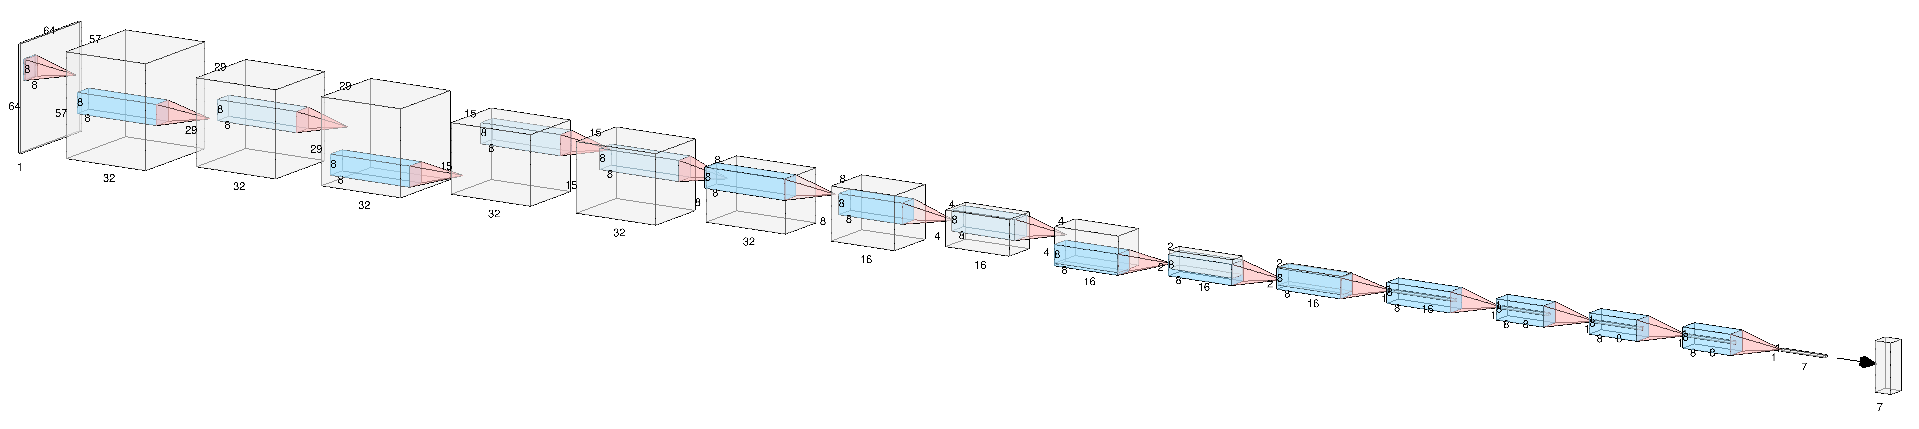
\includegraphics[width=14cm]{gambar/arsitektur_baseline_cnn.png}
    \caption[Arsitektur \acrshort{cnn} \textit{Baseline}]{Arsitektur \acrshort{cnn} \textit{Baseline} \shortcite{agrawal2020using}}
    \label{fig:arsiterturcnnbaseline}
\end{figure}

\textit{Network ensemble} adalah model jaringan yang terdiri beberapa jaringan. Model ini telah terbukti mengungguli model jaringan tunggal. Implementasi model ini mengharuskan tiap-tiap jaringan memiliki keragaman yang cukup dan didukung oleh metode pemaduan yang tepat, yaitu antara lain:
\begin{enumerate}
    \item \textit{Majority voting}: kelas data prediksi ditentukan oleh suara terbanyak dari tiap-tiap jaringan;
    \item \textit{Simple average}: kelas data prediksi ditentukan oleh perhitungan rerata probabilitas dengan bobot yang sama dari tiap-tiap jaringan;
    \item \textit{Weighted average}: kelas data prediksi ditentukan oleh perhitungan rerata probabilitas dengan bobot yang berbeda dari tiap-tiap jaringan \shortcite{li2018deep}.
\end{enumerate}
Model ini diterapkan pada pengenalan ekspresi wajah oleh \shortciteA{kim2016fusing} dan \shortciteA{pramerdorfer2016facial} demi mendapatkan akurasi sebesar 73,73\% dan 75,2\% untuk FER-2013.

\textit{Multitask network} adalah model jaringan yang diusulkan untuk mentransfer pengetahuan dari tugas-tugas relevan dan mengurai faktor-faktor gangguan. Model ini telah digunakan oleh \shortciteA{devries2014multi} dan \shortciteA{zhang2015learning} pada pengenalan ekspresi wajah demi mendapatkan akurasi sebesar 67,21\% dan 75,10\% untuk FER-2013.

\textit{Cascaded network} adalah model jaringan yang memadukan berbagai modul untuk tugas berbeda secara sekuensial. Modul-modul tersebut masing-masing berkontribusi pada penyaringan faktor-faktor variasi berbeda yang tidak dibutuhkan pada pengenalan ekspresi wajah \shortcite{li2018deep}.

\textit{Generative Adversarial Network} (GAN) adalah model jaringan khusus untuk membangkitkan gambar-gambar sintesis yang realistis. Pada pengenalan ekspresi wajah, model ini digunakan oleh \shortciteA{lai2018emotion} untuk membangkitkan gambar wajah frontal dari set data wajah nonfrontal. Penjelasan mendetail tentang model-model jaringan ini dapat ditemukan di \shortciteA{li2018deep}.

Strategi memadukan \acrshort{cnn} dan ekstraksi fitur konvensional belakangan ini telah banyak dilakukan. Strategi ini terbukti dapat meningkatkan akurasi model pengenalan ekspresi wajah. \shortciteA{georgescu2019local}, melalui usaha memadukan fitur-fitur yang diperoleh secara otomatis dan manual, saat ini menjadi \textit{state-of-the-art} bagi pengenalan ekspresi wajah untuk FER-2013. Eksperimen dimulai dengan pemilihan sampel data menggunakan \textit{k-Nearest Neighbor} (k-NN) \shortcite{fix1951discriminatory}. Secara manual, fitur-fitur diperoleh menggunakan model \textit{bag-of-visual-word} (BOVW) \shortcite{ionescu2013local} yang terdiri dari tahap ekstraksi fitur menggunakan \textit{Scale-Invariant Feature Transform} (SIFT) \shortcite{lowe2004distinctive} dan tahap \textit{clustering} menggunakan \textit{k-means} \shortcite{leung2001representing}. Secara otomatis, ekstraksi fitur dilakukan menggunakan tiga model \acrshort{cnn}, yaitu VGG-13 \shortcite{barsoum2016training}, VGG-f \shortcite{chatfield2014return} dan VGG-face \shortcite{parkhi2015deep}. Setelah itu, vektor representasi fitur dari \acrshort{cnn} dan BOVW dirangkai, dinormalisasikan dan dilatih menggunakan model \textit{Dense-Sparse-Dense} (DSD) \shortcite{han2016dsd} dengan \textit{Support Vector Machine} (SVM) \shortcite{cortes1995support} sebagai \textit{classifier}.

\textit{Facial region segmentation} merupakan salah satu teknik \textit{cropping}, yang mana memisahkan beberapa daerah fitur gambar wajah sehingga menghasilkan set data baru (Gambar \ref{fig:segmentasi18}). \textit{Facial region segmentation} telah diterapkan untuk set data wajah frontal karena kelengkapan fitur-fiturnya. Pada \shortciteA{majumder2016automatic}, \textit{facial region segmentation} digunakan untuk memisahkan daerah mata kiri, mata kanan, hidung dan mulut sehingga menghasilkan set data baru. Set data baru tersebut diduplikasi dan dikenakan \textit{local binary pattern} (LBP) \shortcite{ojala1996comparative}. Kemudian set data baru sebelum dan setelah perkenaan LBP dilatih menggunakan \textit{network ensemble} dengan \textit{self-organizing map} (SOM) \textit{classifier} \shortcite{kohonen1990self}. Model tersebut dilatih pada CK+ demi menghasilkan akurasi sebesar 98,95\%. Pada \shortciteA{ye2019facial}, bagian-bagian wajah yang disegmentasi adalah dahi (pertengahan daerah kedua mata), kedua mata dan mulut. Bagian-bagian tersebut dilatih menggunakan \textit{network ensemble} secara individu dan menghasilkan akurasi sebesar 98,70\%.
\begin{figure}[t]
    \centering
    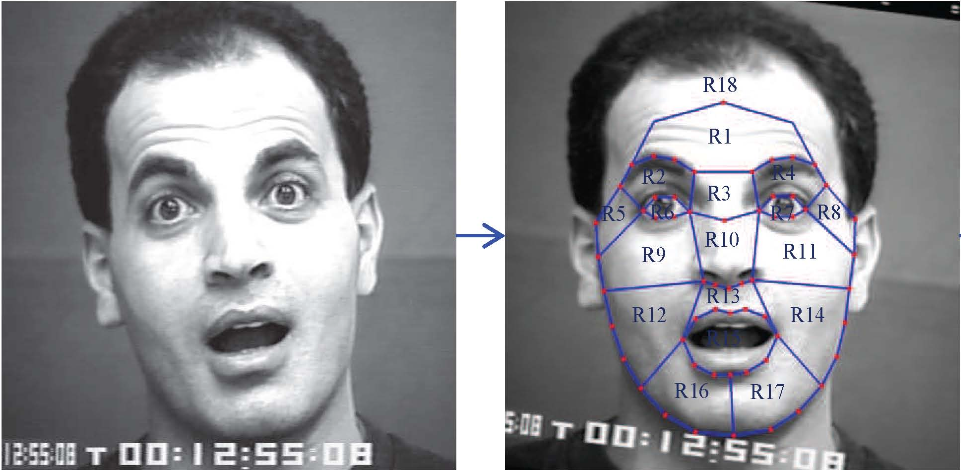
\includegraphics[width=14cm]{gambar/segmentasi_wajah_18.png}
    \caption[Segmentasi Delapan Belas Bagian Wajah]{Segmentasi Delapan Belas Bagian Wajah \protect\shortcite{ghimire2015facial}}
    \label{fig:segmentasi18}
\end{figure}

Filter Gabor merupakan salah satu filter konvolusi \acrshort{2d} yang populer digunakan dalam ekstraksi fitur berbagai tugas klasifikasi gambar menggunakan \acrshort{cnn}. Pada \shortciteA{qin2020facial}, pengenaan sejumlah filter Gabor pada set data input CK+ dibuktikan mampu meningkatkan kemampuan generalisasi \acrshort{cnn} dua kanal dan mencapai akurasi sebesar 96,81\%. Pada \shortciteA{adil2019novel}, penggunaan filter Gabor pada SVM \textit{classifier} menghasilkan akurasi sebesar 92,19\% untuk set data yang sama.

\section{Filter Gabor}
Filter Gabor adalah sebuah filter linear dari fungsi Gabor yang telah berhasil diterapkan di berbagai tugas pemrosesan gambar \shortcite{dunn1993optimal}, misalnya untuk sistem autentikasi biometrik \shortcite{aggrawal2016fingerprint,vijay2019highly}, deteksi kendaraan spesifik \shortcite{sara2019ambulance} dan identifikasi tulisan tangan \shortcite{baati2018towards,mohammed2019handwritten}.

\begin{figure}[t]
    \centering
    \begin{subfigure}[t]{12cm}
        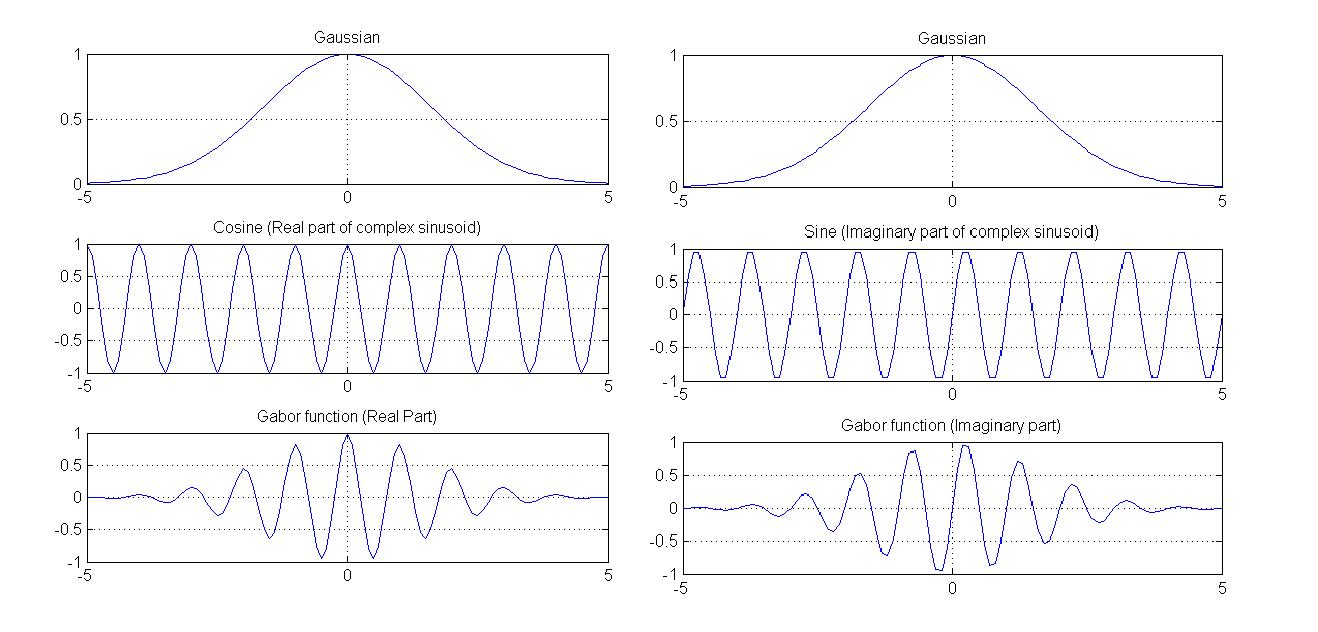
\includegraphics[width=12cm]{gambar/gabor2d.png}
        \caption[Fungsi Gabor pada Dimensi Dua]{Fungsi Gabor pada Dimensi Dua \protect\shortcite{viswanathan2014morlet}}
    \end{subfigure}
    \begin{subfigure}[t]{9cm}
        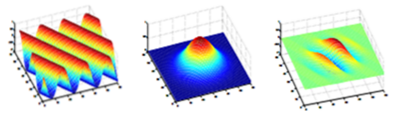
\includegraphics[width=9cm]{gambar/gabor3d.png}
        \caption[Fungsi Gabor pada Dimensi Tiga]{Fungsi Gabor pada Dimensi Tiga (https://medium.com)}
    \end{subfigure}
    ~~~
    \begin{subfigure}[t]{2.8cm}
        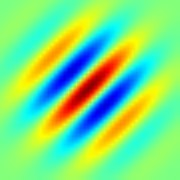
\includegraphics[width=2.8cm]{gambar/filter_gabor.jpg}
        \caption[Filter Gabor]{Filter Gabor (https://think-piece.tistory.com)}
    \end{subfigure}
    \caption[Fungsi Gabor; Hasil Modulasi Sinyal Sinusoidal oleh Fungsi \textit{Gaussian}]{Fungsi Gabor; Hasil Modulasi Sinyal Sinusoidal oleh Fungsi \textit{Gaussian}}
    \label{fig:fungsigabor}
\end{figure}
Fungsi Gabor awalnya diperuntukkan dalam analisis sinyal saluran komunikasi, sebagai fungsi frekuensi terhadap waktu, guna mendapatkan esensi informasi \shortcite{gabor1946theory}. Fungsi ini diperluas menjadi fungsi \acrshort{2d} oleh \shortciteA{daugman1985uncertainty}, sebagai sebuah sinyal sinusoidal kompleks yang dimodulasi oleh fungsi Gaussian (Gambar \ref{fig:fungsigabor}), yang dinyatakan \shortcite{grigorescu20062} dalam (\ref{equ:gabor1}) dan (\ref{equ:gabor2}),
\begin{equation}
    g(x,y,\lambda,\theta,\psi,\sigma,\gamma) = \exp\left(\frac{-x'^2+\gamma^2y'^2}{2\sigma^2}\right) \exp\left(2\pi\frac{x'}{\lambda}+\psi\right)
    \label{equ:gabor1}
\end{equation}
\begin{equation}
    b = \log_2{\left(\frac{\frac{\sigma}{\lambda}\pi+\sqrt{\frac{\ln{2}}{2}}}{\frac{\sigma}{\lambda}\pi-\sqrt{\frac{\ln{2}}{2}}}\right)}, \frac{\sigma}{\lambda} = \frac{1}{\pi}\sqrt{\frac{\ln{2}}{2}}\left(\frac{2^b+1}{2^b-1}\right)
    \label{equ:gabor2}
\end{equation}
dimana,
\begin{description}[align=parleft,labelwidth=1cm]
    \item[$x'$] $= x\cos(\theta) + y\sin(\theta),$
    \item[$y'$] $= -x\sin(\theta) + y\cos(\theta),$
    \item[$\lambda$] $= \parbox[t]{11.3cm}{panjang gelombang faktor cosinus dari fungsi Gabor dengan nilai bilangan riil yang valid 2--256 piksel,}$
    \item[$\theta$] $= \parbox[t]{11.3cm}{orientasi normal terhadap garis paralel fungsi Gabor dengan nilai bilangan riil yang valid 0--80\degree,}$
    \item[$\psi$] $= \parbox[t]{11.3cm}{fase {\itshape offset} faktor kosinus dari fungsi Gabor dengan nilai bilangan riil yang valid -180\degree\ hingga 180\degree,}$
    \item[$\sigma$] $= \parbox[t]{11.3cm}{standar deviasi faktor {\itshape Gaussian} yang nilainya ditentukan oleh parameter $\lambda$ dan $b$,}$
    \item[$\gamma$] $= \parbox[t]{11.3cm}{rasio aspek spasial atau eliptisitas faktor {\itshape Gaussian} dengan nilai terletak antara 0,23 dan 0,92,}$
    \item[$b$] $= \parbox[t]{11.3cm}{{\itshape bandwidth} frekuensi spasial dari filter dengan nilai terletak antara 0,4 dan 2,5 oktaf.}$
\end{description}

Dalam pemrosesan gambar, pertama-tama, bank filter Gabor (Gambar \ref{fig:contohfiltergabor}) dibuat melalui konfigurasi unik berbagai parameter dalam (\ref{equ:gabor1}) dan (\ref{equ:gabor2}). Selanjutnya konvolusi dilakukan melalui perkalian dot matriks antara $m$ filter Gabor dengan $n$ input gambar sehingga menghasilkan $m \times n$ \textit{feature maps} (Gambar \ref{fig:contohkonvolusigabor}).
\begin{figure}
    \centering
    \begin{subfigure}[t]{6.5cm}
        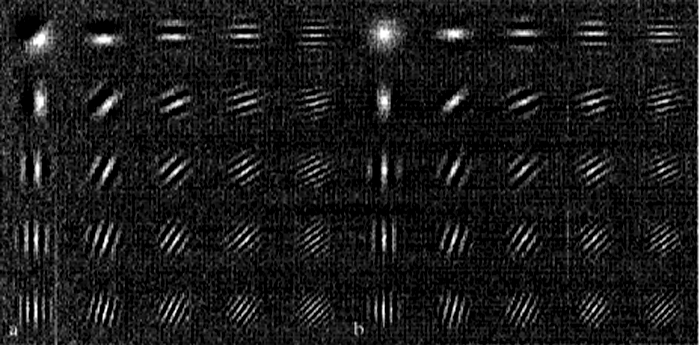
\includegraphics[width=6.5cm]{gambar/filter2_gabor.png}
        \caption[Contoh-Contoh Filter Gabor]{Contoh-Contoh Filter Gabor\\(https://www.cs.auckland.ac.nz)}
        \label{fig:contohfiltergabor}
    \end{subfigure}
    ~~~
    \begin{subfigure}[t]{6cm}
        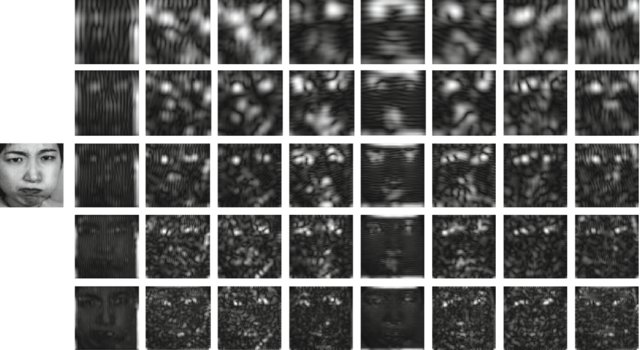
\includegraphics[width=6cm]{gambar/hasil_filter2_gabor.jpg}
        \caption[Contoh-Contoh Hasil Konvolusi oleh Filter Gabor]{Contoh-Contoh Hasil Konvolusi oleh Filter Gabor \protect\shortcite{dahmane2015conditional}}
        \label{fig:contohkonvolusigabor}
    \end{subfigure}
    \caption{Contoh Filter Gabor dan Hasil Konvolusi oleh Filter Gabor}
    \label{fig:konvolusigabor}
\end{figure}

Representasi frekuensi dan orientasi dari filter Gabor ditemukan mirip dengan sistem visual beberapa mamalia, sehingga filter ini sangat cocok untuk analisis tekstur \shortcite{sivalingamaiah2012texture}. Oleh karena itu, komputasi transformasi kompleks sebab tidak ortogonal menjadi kelemahan utama filter ini. Sifatnya yang demikian menimbulkan redudansi koefisien dan informasi \shortcite{vyas2006automated}. Sehingga tidak cocok digunakan pada sistem waktu nyata. Hal ini memotivasi berbagai penelitian untuk mencoba melakukan optimasi tanpa kehilangan akurasi yang berarti (\shortciteNP{ilonen2005efficient}; \shortciteNP{amayeh2009accurate}; \shortciteNP{kugaevskikh2017comparison}).

\section{Filter Log-Gabor}
\shortciteA{nava2011comparison} menyebutkan bahwa fungsi log-Gabor \shortcite{field87} dapat mengungguli performa fungsi Gabor pada pengenalan gambar yang memiliki tekstur yang kompleks. Dengan asumsi bahwa ekspresi wajah terbentuk dari kombinasi berbagai otot wajah yang menghasilkan tekstur kulit wajah yang kompleks, fungsi log-Gabor diharapkan dapat meningkatkan performa model rekognisi emosi. Fungsi log-Gabor dapat dirumuskan \shortcite{walia2016boosting} ke dalam (\ref{equ:loggabor}),
\begin{equation}
    g(r,\theta) = \exp{\left(\frac{-\log^2{\left(\frac{r}{f_0}\right)}}{2\sigma^2_r}\right)} \exp{\left(\frac{-(\theta-\theta_0)^2}{2\sigma^2_\theta}\right)},
    \label{equ:loggabor}
\end{equation}
% \begin{center}
%     dengan
% \end{center}
\begin{equation}
    f_0 = \text{wav}\times\text{scaleFactor}^n
\end{equation}
dimana,
\begin{description}[align=parleft,labelwidth=2cm]
    \item[$(r, \theta)$] $= \parbox[t]{10.3cm}{koordinat polar}$
    \item[$f_0$] $= \parbox[t]{10.3cm}{frekuensi pusat filter}$
    \item[\normalfont{wav}] $= \parbox[t]{10.3cm}{panjang gelombang dari skala terkecil}$
    \item[\normalfont{scaleFactor}] $= \parbox[t]{10.3cm}{faktor skala antar filter terurut}$
    \item[$\theta$] $= \parbox[t]{10.3cm}{sudut orientasi filter}$
    \item[$\sigma_r$] $= \parbox[t]{10.3cm}{skala {\itshape bandwidth}}$
    \item[$\sigma_\theta$] $= \parbox[t]{10.3cm}{sudut {\itshape bandwidth}}$
\end{description}

% TODO: contoh filter log-gabor

\section{\textit{\acrlong{ml}}}
\textit{Learning} adalah fenomena ---yang disimpulkan dari perilaku--- yang dapat diamati di seluruh makhluk hidup, termasuk manusia, hewan \shortcite{beran2020animal} dan tanaman \shortcite{parise2020extended}, baik saat mereka terjaga maupun saat tidur. \textit{Learning} dapat terjadi sekalipun tanpa keterlibatan dari orang lain \shortcite{gross2015psychology}. \textit{Learning} berarti perubahan potensi perilaku yang relatif permanen akibat keteraturan di lingkungan pelaku \shortcite{de2013learning,haselgrove2016learning}.

Hewan dan tanaman belajar melalui hubungan antara peristiwa dan respons yang berdekatan (\textit{associative learning}). Sebagai contoh, seekor kucing yang mana selalu diberi makan oleh pemiliknya setiap kali mengeong di dapur belajar jika mengeong adalah cara untuk meminta dan mendapatkan makanan \shortcite{ramos2009animal}. Contoh lain, tanaman putri malu akan mengatup sedikit dalam menanggapi sentuhan ringan dan akan mengatup rapat dalam menanggapi stimulus taktil. Setelah beberapa kali dikenakan sentuhan ringan dan stimulus taktil, maka tanaman putri malu akan mulai mengatup rapat dalam menanggapi sentuhan ringan \shortcite{abramson2016learning}.

\textit{Machine learning} \shortcite{hebb1949organization} muncul akibat keinginan untuk mengenakan \textit{learning} kepada mesin, sehingga dia mampu berinteraksi dengan lingkungannya berdasarkan pengetahuan yang diperoleh dari pengalaman. Untuk itu, berbagai disiplin terkait dipelajari seperti statistika, model interaksi sel-sel otak, teori kontrol adaptif, model-model psikologi, kecerdasan buatan, dan model-model evolusi \shortcite{nilsson2005introduction}. Akan tetapi, bagaimanapun, hingga saat ini, konsep-konsep dan teknik-teknik \textit{machine learning} lebih banyak diperoleh dari statistika daripada disiplin lain \shortcite{mitchell2006discipline}.

Sebuah mesin dikatakan belajar jika sistem secara andal meningkatkan kinerja (yang diukur oleh metrik tertentu) secara otomatis pada tugas tertentu mengikuti pengalaman tertentu. Mesin tersebut harus mampu bekerja menurut arsitektur komputasi dan algoritma tertentu dalam memproses set data statistik untuk aplikasi dimana \shortcite{nilsson2005introduction,mitchell2006discipline}:
\begin{enumerate}
    \item Beberapa tugas memerlukan algoritma yang rumit untuk didesain secara manual. Atau dengan kata lain, hanya dapat ditentukan oleh pasangan input dan keluaran. Sebagai contoh, tidak ada seorang pun mampu menulis algoritma untuk melabeli foto-foto yang memuat dirinya, namun melakukannya adalah mudah bagi semua orang.
    \item Korelasi antar data tersembunyi dalam himpunan data yang besar dan kompleks. Sebagai contoh, pada kasus penipuan kartu kredit, akan sangat sulit bagi orang untuk menemukan pola penipuan secara manual dari data transaksi bank.
    \item Lingkungan operasional tidak terdefinisi secara komplet pada waktu desain. Sebagai contoh, toko buku daring yang mampu menyesuaikan diri dengan preferensi pembelian setiap akun pelanggan.
\end{enumerate}
Dengan syarat-syarat di atas, pemanfaatan \textit{machine learning} menjadi sangat luas dan beragam. \textit{Machine learning} dapat diterapkan dengan bijak hampir di setiap lini kehidupan manusia.

% \textit{Machine learning} tidak terbatas oleh masalah-masalah dengan bentukan data input tertentu. Sebaliknya, dia menerima hampir semua data konkret, mencakup data vektor, \textit{list}, set, matrix, gambar, video, graf, \textit{string} dan campuran dari itu semua \shortcite{smola2008introduction}. Tiap-tiap jenis data tersebut diolah dengan cara-cara yang berbeda.

% \begin{figure}
%     \centering
%     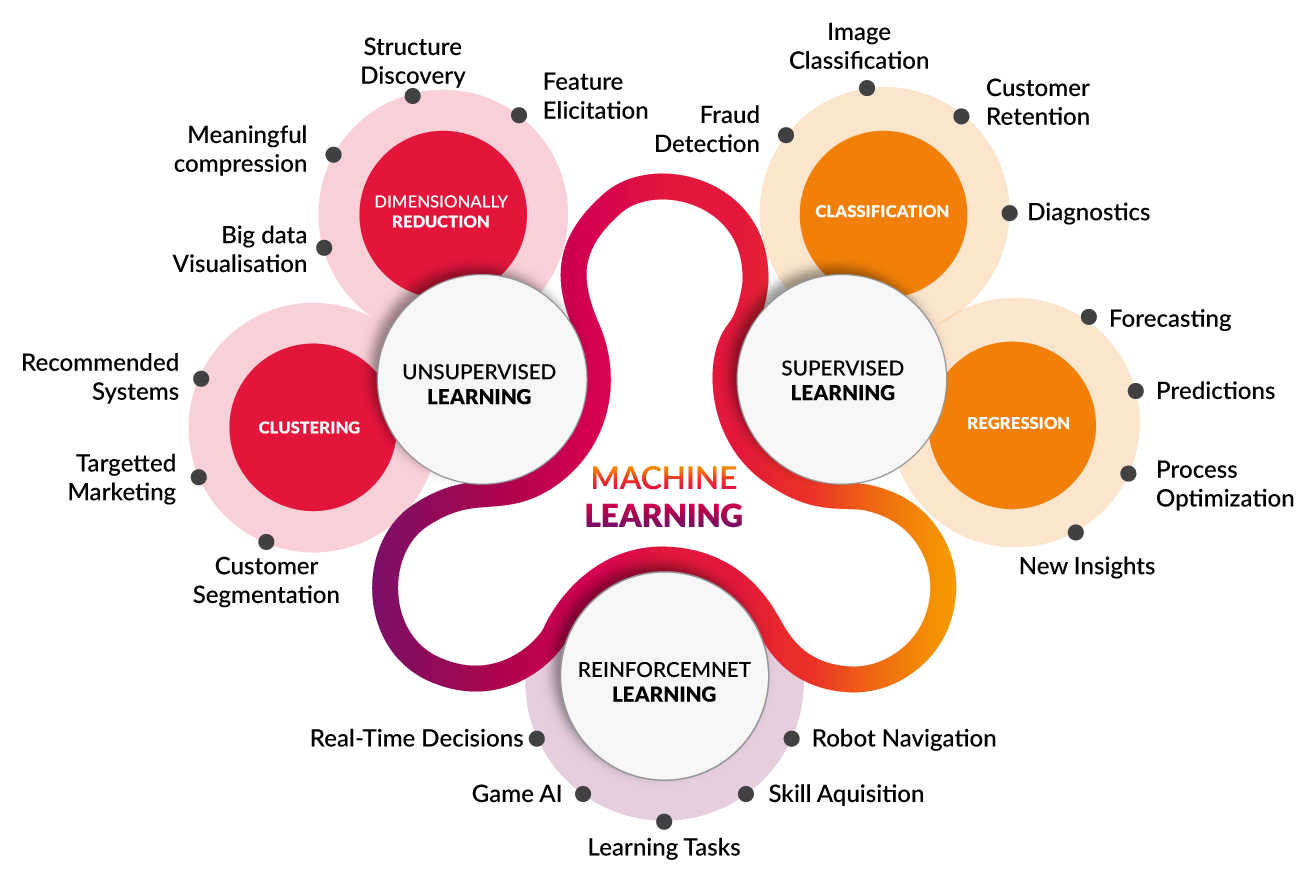
\includegraphics[width=12cm]{gambar/machine_learning_task.png}
%     \caption[Klasifikasi \textit{Machine Learning}]{Klasifikasi \textit{Machine Learning}\\(https://www.cognub.com)}
%     \label{fig:klasifikasiml}
% \end{figure}
% Tugas-tugas \textit{machine learning} dapat dibedakan menjadi \textit{supervised learning}, \textit{unsupervised learning} dan \textit{reinforcement learning} (Gambar \ref{fig:klasifikasiml}). \dots

% Problem-problem \textit{supervised learning}, berdasarkan keluarannya, dapat dibedakan menjadi klasifikasi dan regresi. Problem-problem klasifikasi, berdasarkan jumlahnya, dapat dibedakan menjadi \textit{binary classification} dan \textit{multiclass classification}. \dots

\subsection{\textit{\acrlong{ann}}}
\begin{figure}[t]
    \centering
    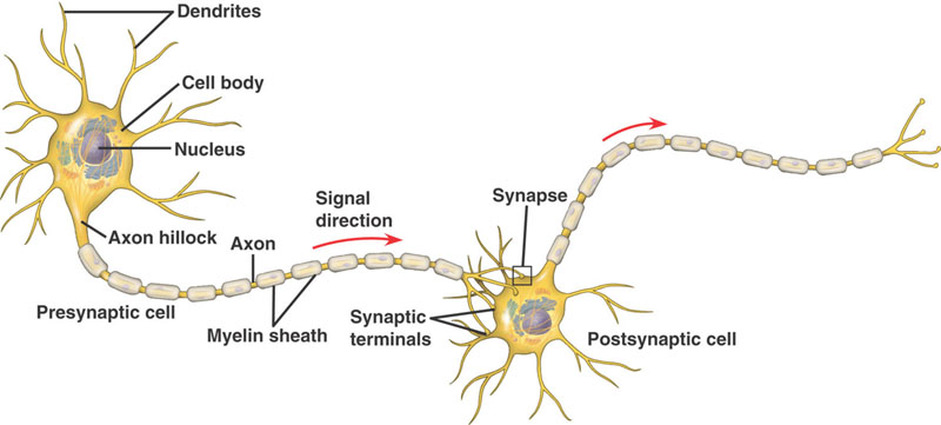
\includegraphics[width=10cm]{gambar/neuron.jpg}
    \caption[Struktur Neuron]{Struktur Neuron (https://mikerbio.weebly.com)}
    \label{fig:neuron}
\end{figure}
Otak manusia tersusun atas miliaran neuron yang saling berhubungan. Masing-masing neuron memiliki sel tubuh (soma), sejumlah dendrit dan sejumlah akson (Gambar \ref{fig:neuron}). Dendrit berfungsi untuk menerima sinyal dari akson lain pada neuron tetangga. Sinyal tersebut akan ditransmisikan melalui dari akson ke dendrit yang terkoneksi melalui sinapsis jika kekuatan sinyal tersebut di atas ambang batas tertentu. Melalui penyebaran dan interaksi sinyal-sinyal ini dalam anatomi neuron yang rumit, di mana melibatkan mekanisme nonlinear pada berbagai skala temporal dan spasial, pemrosesan informasi di otak berlangsung \shortcite{hines1997neuron,singh2001introduction}.

\textit{\acrlong{ann}} (\acrshort{ann}) mengacu pada model matematika yang memiliki arsitektur terdistribusi, yaitu terdiri atas soma (dapat dianalogikan) sebagai simpul/unit komputasi, sejumlah dendrit sebagai input, sejumlah akson sebagai keluaran dan sinapsis sebagai penyimpan informasi berupa bobot/parameter. Setiap simpul memiliki sebuah fungsi tertentu yang disebut \textit{perceptron} \shortcite{singh2001introduction,an2017electrical}. Secara umum, jaringan ini dapat digambarkan sebagai graf terarah yang terdiri dari lapisan input, lapisan tersembunyi dan lapisan target. Lapisan input terdiri dari $i$ buah simpul ditambah dengan sebuah simpul konstan yang selalu menghasilkan nilai bobot sama dengan satu. Di mana lapisan tersembunyi dapat terdiri dari satu atau lebih lapisan yang memiliki sejumlah simpul yang saling terhubung. Setiap lapisan tersembunyi dapat memiliki jumlah simpul yang beragam ditambah sebuah simpul bias yang tidak memiliki input dan menghasilkan sebuah konstanta. Kedalaman jaringan diukur dengan menjumlahkan banyak lapisan tersembunyi dan lapisan target. Besar jaringan diukur dengan menjumlahkan seluruh simpul pada setiap lapisan jaringan \shortcite{shalev2014understanding}.

\begin{figure}
    \centering
    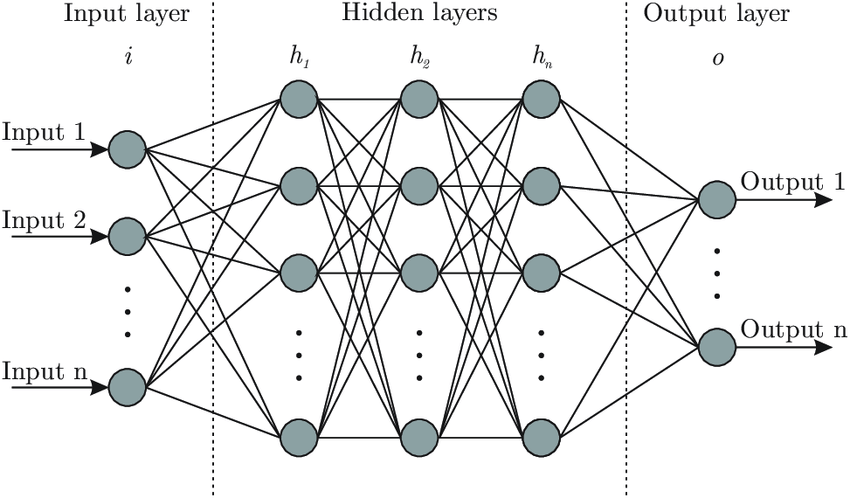
\includegraphics[width=10cm]{gambar/model_ann.png}
    \caption[Model \textit{\acrlong{ann}}]{Model \textit{\acrlong{ann}} \protect\shortcite{bre2018prediction}}
    \label{fig:modelann}
\end{figure}
Salah satu bentuk dari jaringan ini adalah \textit{feedforward multilayer perceptron}, di mana \textit{feedforward} berarti aliran data bergerak satu arah, dari input ke target/keluaran. Gambar \ref{fig:modelann} memperlihatkan jaringan \textit{feedforward} yang memiliki sejumlah input, tiga lapisan tersembunyi dan sejumlah target. Misalkan ($x_1, x_2, ..., x_i$) merupakan vektor input dan ($y_1, y_2, ..., y_m$) merupakan vektor target. Setiap simpul input terkoneksi dengan setiap simpul pada lapisan tersembunyi pertama dan setiap koneksi ini memiliki sebuah bobot $w_{i,j}$. Maka simpul ke-$j$ pada lapisan tersembunyi pertama, melalui fungsi aktivasi/transfer nonlinear tanh, melewatkan hasil penjumlahan bobot dari setiap inputnya, yaitu
\begin{equation}
    p_j = \tanh \left(\sum_i{w_{i,j}x_i}\right)
    \label{equ:hd1}
\end{equation}
Melalui proses yang sama, keluaran setiap simpul pada lapisan tersembunyi kedua dan ketiga berturut-turut adalah
\begin{equation}
    q_k = \tanh \left(\sum_j{w_{j,k}x_j}\right)
    \label{equ:hd2}
\end{equation}
\begin{equation}
    r_l = \tanh \left(\sum_k{w_{k,l}x_k}\right)
    \label{equ:hd3}
\end{equation}
Akhirnya, lapisan target melakukan penjumlahan sederhana dari setiap inputnya dengan
\begin{equation}
    y_m = \sum_l{w_{l,m}x_l}
    \label{equ:ol}
\end{equation}
Fungsi tanh dapat digantikan oleh fungsi nonlinear lain, misalnya fungsi sigmoid: $1/(1-\exp{\left[-\sum{wx}\right]})$. Kedua fungsi ini memetakan rentang input yang tidak terbatas ke rentang keluaran terbatas \shortcite{singh2001introduction}.

\textit{Supervised learning} melatih jaringan dengan menginterpolasi data pelatihan untuk memberikan generalisasi hubungan antar set data input dan target. Sebab hampir tidak mungkin untuk memperoleh hubungan yang konvergen di hampir setiap kasus. Interpolasi dilakukan melalui penyesuaian setiap nilai bobot sebanyak $n$ \textit{epoch} atau hingga mencapai model yang optimal. Model optimal diperoleh dengan meminimalkan fungsi eror untuk semua bobot jaringan. Di antara fungsi tersebut adalah fungsi eror \textit{sum-of-squares}, yaitu \shortcite{singh2001introduction}
\begin{equation}
    e^{\{z\}} = \frac{1}{2}\sum_m{\beta(y^{\{z\}}_m-T^{\{z\}}_m)^2}
    \label{equ:sos}
\end{equation}
dimana,
\begin{description}[align=parleft,labelwidth=1cm]
    \item[$z$] $= \parbox[t]{10.35cm}{input vektor tunggal}$
    \item[$T_m$] $= \parbox[t]{10.35cm}{nilai keluaran target}$
    \item[$m$] $= \parbox[t]{10.35cm}{indeks simpul target}$
    \item[$\beta_m$] $= \parbox[t]{10.35cm}{nilai prioritas bobot}$
\end{description}

\textit{Backpropagation} \shortcite{rumelhart1986learning} merupakan salah satu algoritma populer untuk melatih jaringan dengan menentukan gradien fungsi eror tiap-tiap bobot. Bobot-bobot ini mulanya diinisialisasi dengan nilai acak kecil. Dalam kalkulus, gradien garis singgung sebuah fungsi nonlinear di sebuah titik dapat diperoleh melalui subtitusi nilai koordinat titik tersebut ke dalam derivatif/turunan parsial fungsi nonlinear tersebut \shortcite{shalev2014understanding}. Pada lapisan bobot target, dengan mensubstitusikan (\ref{equ:ol}) ke dalam (\ref{equ:sos}), gradien fungsi eror setiap bobot diperoleh dari
\begin{equation}
    \frac{\partial e}{\partial w_{k,l}} = \sum_m{\beta(y_m - T_m) \frac{\partial y_m}{\partial w_{k,l}}} = \frac{\partial r_l}{\partial w_{k,l}} \sum_m{\beta(y_m - T_m) w_{l,m}}
\end{equation}
Proses perhitungan ini berlanjut dari lapisan bobot target ke lapisan-lapisan bobot tersembunyi sehingga memberikan vektor gradien eror komplit, ${\partial e}/{\partial w}$, di mana $w$ adalah set seluruh bobot jaringan. Evaluasi vektor gradien eror ini dapat dilakukan melalui proses \textit{gradien descent}, yaitu dengan menyesuaikan vektor bobot ke arah negatif terhadap vektor gradien, contohnya
\begin{equation}
    \Delta w = -\mu\frac{\partial e}{\partial w}
\end{equation}
di mana $\mu$ adalah besaran langkah yang diambil yang umumnya bernilai 0,1--1,0. Gradien ini dihitung ulang menggunakan nilai bobot yang baru sebanyak $n$ \textit{epoch} atau hingga mencapai nilai eror mendekati nol. Nilai bobot yang baru akan diperbarui setiap kali vektor dari set data pelatihan melewati sebuah simpul. Untuk mengurangi waktu yang diperlukan dalam memperbarui setiap nilai bobot, pelatihan \textit{batch} dipraktikkan, yaitu dengan memperbarui setiap nilai bobot hanya setelah mendapatkan rerata eror untuk seluruh vektor tersebut,
\begin{equation}
    E = \frac{1}{Z} \sum_{z=1}^{z=Z}{e^{\{z\}}}
\end{equation}
dan vektor gradien eror yang bersesuaian \shortcite{singh2001introduction}.

Dalam konteks permasalahan pada penelitian ini, penulis menggunakan \textit{loss function} yaitu \textit{categorical crossentropy} yang cocok untuk klasifikasi multikelas (jumlah kelas $>$ 2) berlabel tunggal pada kasus ini. Untuk itu, aktivasi \textit{softmax} \shortcite{grave2016m} digunakan pada lapisan terakhir pada jaringan. Fungsi \textit{softmax} didefinisikan oleh (\ref{equ:lossfunc}),
\begin{equation}
    f(z_w) = \frac{\exp{(z_w)}}{\mathlarger{\sum}\limits_{w' \in V}{\exp{(z_{w'})}}}
    \label{equ:lossfunc}
\end{equation}
dimana,
\begin{description}[align=parleft,labelwidth=1cm]
    \item[$z_w$] $= \parbox[t]{10.9cm}{representasi kelas yang dihitung}$
    \item[$z_w'$] $= \parbox[t]{10.9cm}{representasi kelas selain yang dihitung}$
    \item[$w$] $= \parbox[t]{10.9cm}{kelas yang dihitung}$
    \item[$w'$] $= \parbox[t]{10.9cm}{kelas selain yang dihitung}$
    \item[$V$] $= \parbox[t]{10.9cm}{himpunan kelas}$
\end{description}
\textit{Softmax} bekerja dengan menentukan probabilitas sebuah kasus untuk setiap kelas prediksi. Nilai probabilitas tersebut berkisar antara 0 dan 1. Jika semua probabilitas dijumlahkan maka akan sama dengan 1.

Sementara itu, \textit{learning rate} diperoleh menggunakan \textit{\acrlong{adam}} (\acrshort{adam}), yang merupakan peningkatan dari metode \textit{Gradient Descent} standar, sebagai \textit{optimizer}. \acrshort{adam} bekerja dengan menghitung \textit{learning rate} yang adaptif untuk setiap parameter \shortcite{prilianti2019performance}. \acrshort{adam} dipilih bukan berarti paling optimal, melainkan karena lebih mudah dikonfigurasi \shortcite{schneider2019deepobs}. \acrshort{adam} dapat diformulasikan ke dalam (\ref{equ:adama})--(\ref{equ:adame}),
\begin{equation}
    m_t = \beta_1m_{t-1}+(1-\beta_1)g_t
    \label{equ:adama}
\end{equation}
\begin{equation}
    \hat m_t = \frac{m_t}{1-\beta^t_1}
    \label{equ:adamb}
\end{equation}
\begin{equation}
    v_t = \beta_2v_{t-1}+(1-\beta_2)g_t
    \label{equ:adamc}
\end{equation}
\begin{equation}
    \hat v_t = \frac{v_t}{1-\beta^t_2}
    \label{equ:adamd}
\end{equation}
\begin{equation}
    \theta_{t-1} = \theta_t-\frac{\eta}{\sqrt{\hat v_t + \epsilon}} \hat m_t
    \label{equ:adame}
\end{equation}
dimana,
\begin{description}[align=parleft,labelwidth=1.5cm]
    \item[$\hat v_t$] $= \parbox[t]{9.9cm}{gradien kuadrat sebelumnya dengan bias yang dikoreksi}$
    \item[$\hat m_t$] $= \parbox[t]{9.9cm}{gradien rata-rata sebelumnya dengan bias yang dikoreksi}$
    \item[$v_t, m_t$] $= \parbox[t]{9.9cm}{keduanya memperkirakan peluruhan momen pertama dan kedua dari gradien yang dihitung}$
    \item[$\beta$] $= \parbox[t]{9.9cm}{konstanta peluruhan}$
    \item[$\theta_{t+1}$] $= \parbox[t]{9.9cm}{Parameter pembaruan untuk $t+1$}$
\end{description}

\subsection{\textit{\acrlong{cnn}}}
Pengenalan tulisan tangan merupakan sebuah permasalahan klasik pada topik irisan antara \textit{machine learning} dan \textit{computer vision}, di mana pengaplikasian \acrshort{ann} untuk kasus ini menghadapi dua tantangan besar. Secara sederhana, \acrshort{ann} dapat menerima set data input berlabel manapun selama itu valid dan representatif untuk kemudian melatih model yang secara umum mampu mengenali bentuk tulisan apapun. Dalam kasus ini, set data input yang digunakan adalah berupa set matriks dua dimensi yang mengandung setiap piksel dari sebuah data gambar. Sesuai dengan sifat dari matriks, transformasi geometri tertentu dimungkinkan terjadi sehingga akan memperbanyak kondisi yang perlu ditangani oleh jaringan. Sebagai akibatnya, set data \textit{learning} yang diperlukan menjadi sangat banyak dan variatif. Untuk kasus pengenalan yang lebih rumit, pengumpulan data akan menjadi semakin mustahil dilakukan. Dalam konteks pemrosesan gambar, setiap piksel merupakan representasi dari makna yang terkandung dalam sebuah gambar. Oleh karena itu, setiap piksel dari setiap data gambar input akan dimasukkan sebagai inputan jaringan. Semakin besar ukuran piksel dan semakin banyak data gambar input akan membuat proses pelatihan model memerlukan semakin banyak waktu dan semakin besar memori.

Untuk menjawab tantangan di atas, \shortciteA{lecun1989generalization} memperkenalkan sebuah jaringan spesial yang secara statistik terbukti lebih andal dalam memproses set data gambar, yaitu \textit{\acrlong{cnn}} (\acrshort{cnn}). Sesuai dengan sebutannya, jaringan ini mengharuskan terjadinya proses konvolusi minimal di salah satu lapisan tersembunyi. Secara umum, konvolusi adalah sebuah operasi perkalian matematika terhadap dua buah matriks dengan aturan dan parameter tertentu. Konvolusi \acrshort{1d} dapat didefinisikan oleh,
\begin{equation}
    y(t) = \int{x(a)w(t-a)}\,\mathrm{d}a
\end{equation}
di mana $t$ adalah indeks waktu dan $a$ adalah umur pengukuran. Konvolusi biasanya dinotasikan dengan lambang bintang (\textit{asterisk}):
\begin{equation}
    y(t) = (x \ast w)(t)
\end{equation}
di mana fungsi $x$ adalah input, fungsi $w$ adalah bobot/kernel dan fungsi $y$ adalah peta fitur/\textit{feature map}. Sementara waktu $t$ diasumsikan dengan nilai integer, maka konvolusi diskrit didefinisikan sebagai,
\begin{equation}
    y(t) = (x \ast w)(t) = \sum_{a=-\infty}^{\infty}{x(1)w(t-a)}
\end{equation}
Input di sini pada umumnya adalah larik data multidimensi, sedangkan kernel adalah larik bobot multidimensi. Larik multidimensi ini sering disebut sebagai tensor. Konvolusi \acrshort{2d} dapat ditulis sebagai,
\begin{equation}
    Y(i,j) = (I \ast K)(i,j) = \sum_m{\sum_n{I(m,n)K(i-m,j-n)}}
\end{equation}
di mana $I$ adalah larik gambar \acrshort{2d} dan $K$ adalah larik kernel \acrshort{2d}. Konvolusi ini bersifat komutatif akibat pembalikan larik kernel guna mendapatkan pembuktian. Namun, hal ini tidak penting dalam implementasi \acrshort{ann}. Sehingga banyak pustaka \acrshort{ann} mengimplementasikan \textit{cross-correlation}, konvolusi tanpa membalikkan kernel, dan menyebutnya sebagai konvolusi \shortcite{goodfellow2013challenges}:
\begin{equation}
    Y(i,j) = (K \ast I)(i,j) = \sum_m{\sum_n{K(i+m,j+n)I(m,n)}}
\end{equation}

\begin{figure}
    \centering
    \begin{subfigure}[t]{14cm}
        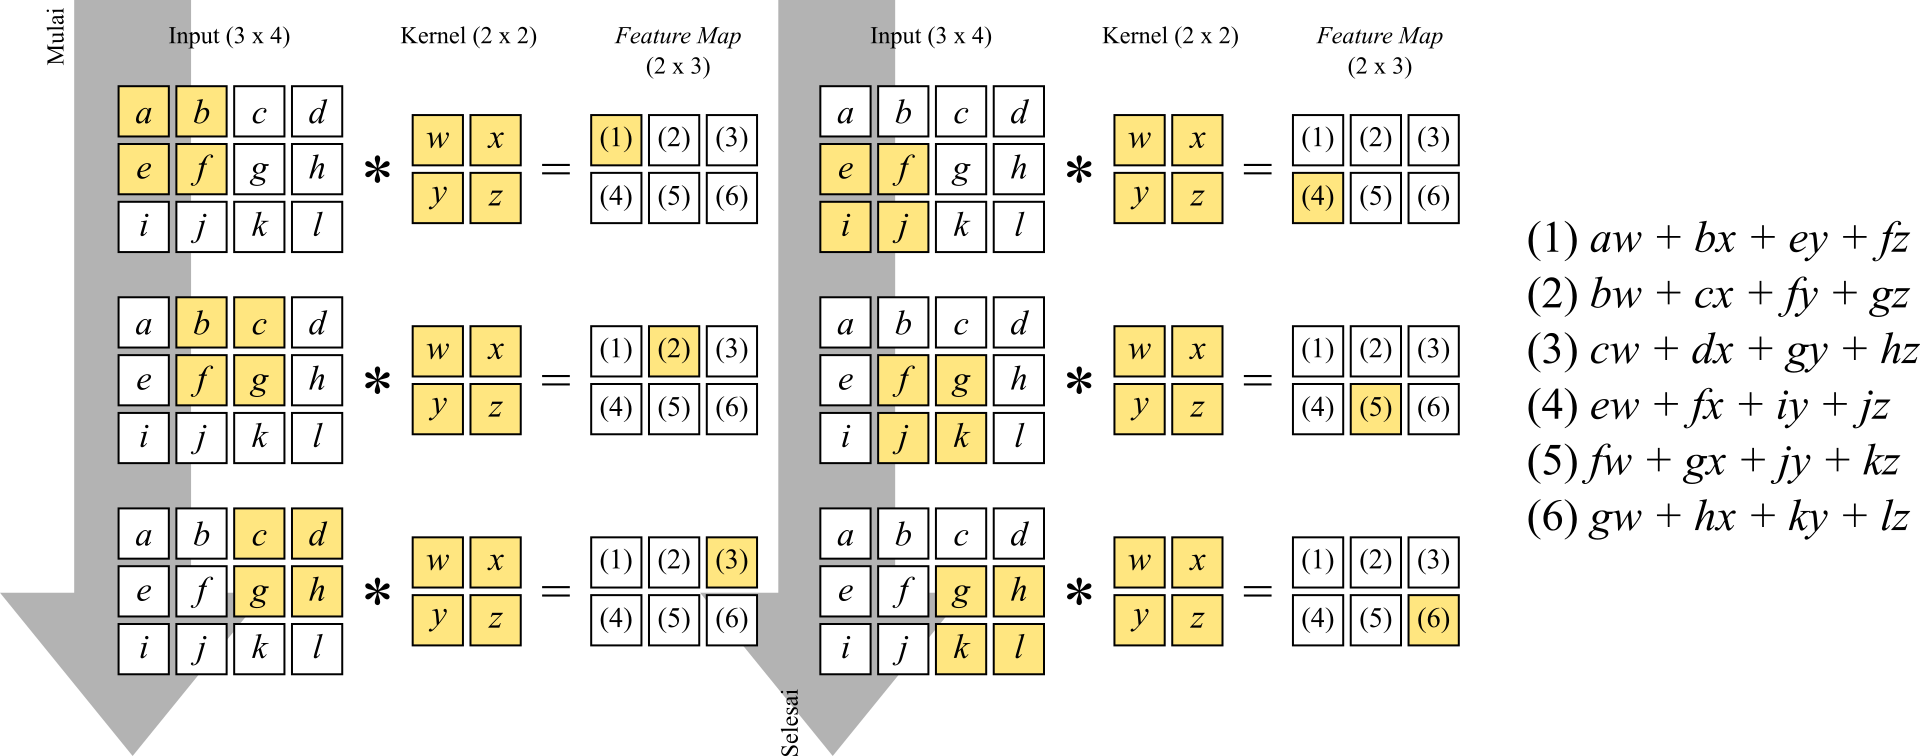
\includegraphics[width=14cm]{gambar/contoh_konvolusi1.png}
        \caption{\footnotesize Konvolusi \acrshort{2d} oleh Kernel $2 \times 2$ dengan \textit{Stride} $1 \times 1$ tanpa \textit{Zero Padding}}
        \label{fig:konvolusi1}
    \end{subfigure}
    \begin{subfigure}[t]{14cm}
        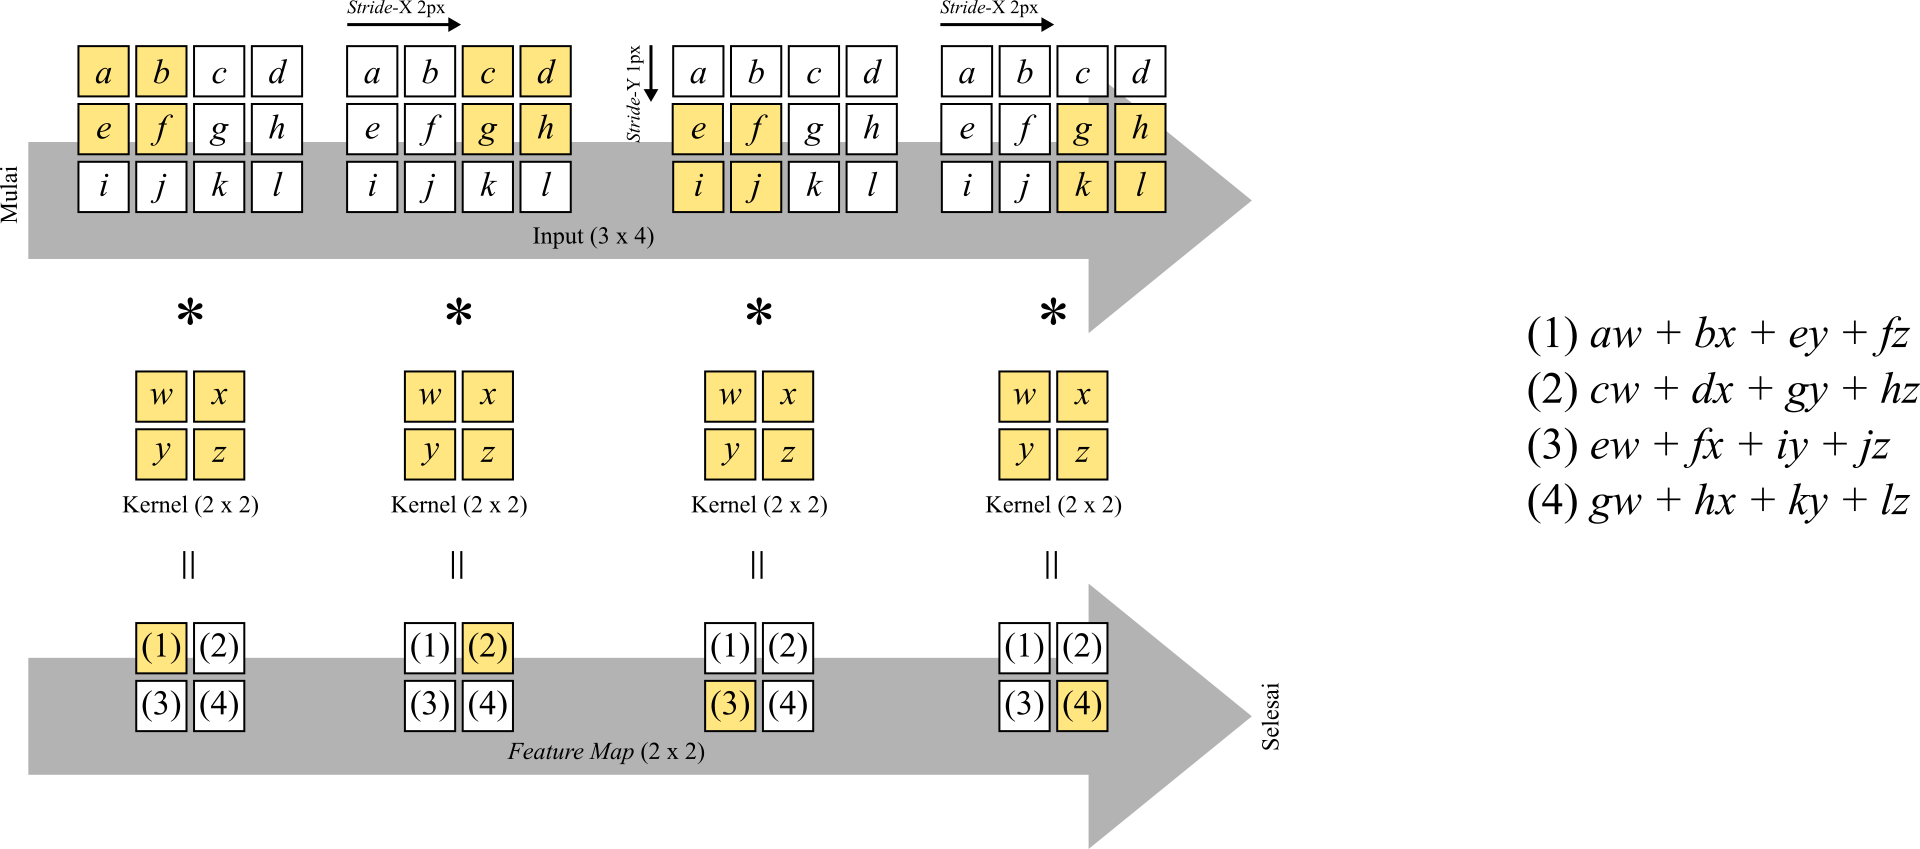
\includegraphics[width=14cm]{gambar/contoh_konvolusi2.png}
        \caption{\footnotesize Konvolusi \acrshort{2d} oleh Kernel $2 \times 2$ dengan \textit{Stride} $2 \times 1$ tanpa \textit{Zero Padding}}
        \label{fig:konvolusi2}
    \end{subfigure}
    \begin{subfigure}[t]{14cm}
        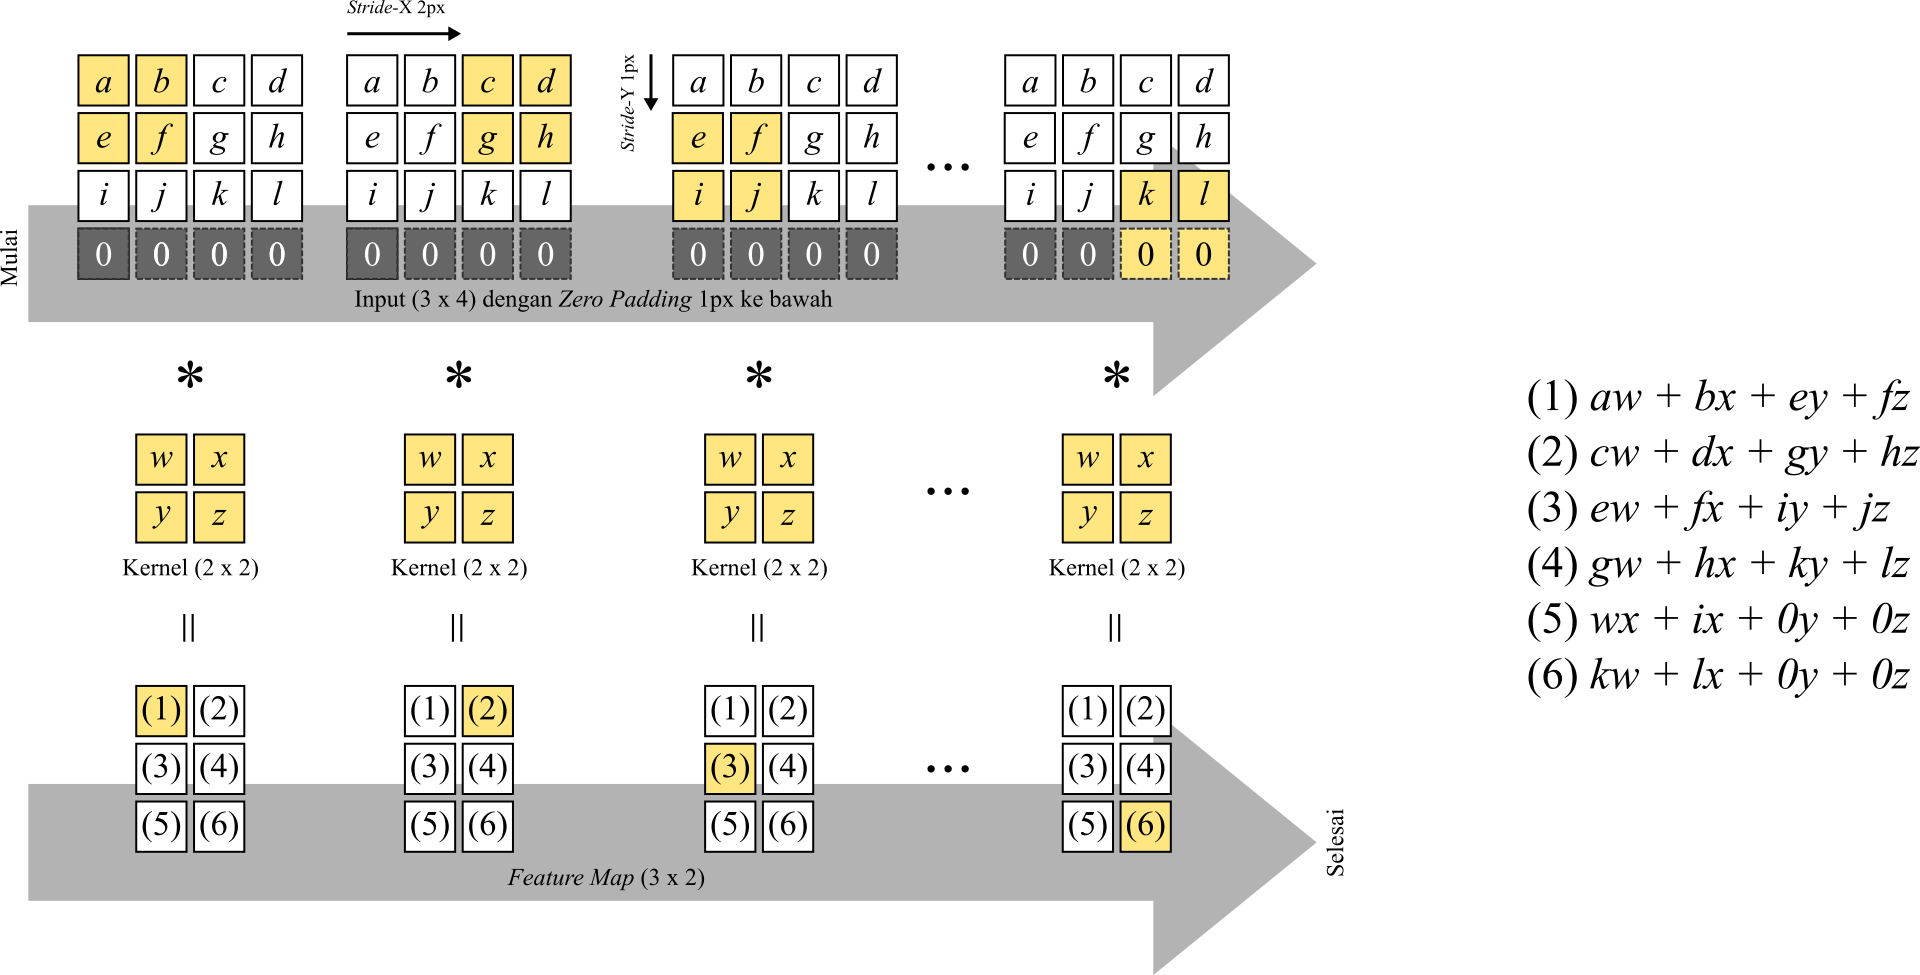
\includegraphics[width=14cm]{gambar/contoh_konvolusi3.png}
        \caption{\footnotesize Konvolusi \acrshort{2d} oleh Kernel $2 \times 2$ dengan \textit{Stride} $2 \times 1$ dan \textit{Zero Padding}}
        \label{fig:konvolusi3}
    \end{subfigure}
    \caption[Kasus-Kasus Konvolusi \acrshort{2d}]{Kasus-Kasus Konvolusi \acrshort{2d} \protect\shortcite{goodfellow2016deep}}
    \label{fig:contoh_konvolusi}
\end{figure}
Gambar \ref{fig:konvolusi1} memperlihatkan contoh konvolusi input $I(3,4)$ oleh kernel $K(2,2)$ menghasilkan \textit{feature map} $F(2,3)$. \acrshort{cnn} biasanya memiliki interaksi atau konektivitas \textit{sparse} ketika ukuran kernel lebih kecil daripada ukuran input. Tujuannya adalah mengurangi jumlah memori yang dibutuhkan untuk menyimpan parameter-parameter dari fitur-fitur gambar yang berarti. Jika ukuran kernel diperbesar, maka ukuran \textit{feature map} akan lebih kecil. Dan begitu pula sebaliknya. Di lapangan, konvolusi memiliki parameter tambahan yang disebut sebagai \textit{stride}, yang mana parameter ini mengatur seberapa besar pergeseran operasi perkalian oleh kernel terhadap input. \textit{Stride} yang berukuran lebih besar akan menghasilkan \textit{feature map} yang lebih kecil. Gambar \ref{fig:konvolusi2} menunjukkan bagaimana ukuran \textit{stride} yang berbeda, dari contoh pada Gambar \ref{fig:konvolusi1}, dapat mempengaruhi pemetaan dari input ke \textit{feature map} melalui proses konvolusi. Pemetaan dari input ke \textit{feature map} tanpa penambahan apapun terhadap input sering disebut sebagai konvolusi yang valid. Kita juga dapat mengendarai ukuran \textit{feature map} dengan melakukan zero padding pada input, di mana input diperluas dengan menambahkan aksis tertentu yang semua pikselnya bernilai nol seperti yang ditunjukkan pada Gambar \ref{fig:konvolusi3} \shortcite{goodfellow2016deep}.

Praproses data merupakan tahap yang cukup penting untuk pemodelan klasifikasi gambar. Praproses harus dilakukan secara hati-hati melalui analisis karakteristik data inputan. Pemilihan praproses yang tepat menghasilkan tahap ekstraksi fitur yang lebih baik. Sebaliknya, pemilihan yang tidak tepat dapat merusak atau bahkan menghilangkan fitur. Beragam praproses telah diterapkan oleh penelitian-penelitian terkait terdahulu, di antaranya adalah \textit{data augmentation}, \textit{illumination normalization}, \textit{face alignment} dan \textit{pose normalization}.

% TODO: histogram equalization

\textit{\acrlong{zca}} (\acrshort{zca}) merupakan teknik \textit{image whitening} yang terbukti mengungguli performa model klasifikasi gambar yang dikenakan oleh teknik normalisasi rerata dan standarisasi piksel gambar. Beberapa contoh hasil penggunaan teknik ini ditunjukkan pada Gambar \ref{fig:contohhasilzca}. Sementara fungsi \acrshort{zca} \shortcite{pal2016preprocessing} dijelaskan pada (\ref{equ:zca}),
\begin{equation}
    X_{\text{ZCA}} = U.\text{diag}(1/\sqrt{\text{diag}(S)+\epsilon}).U^T.X'
    \label{equ:zca}
\end{equation}
\begin{equation}
    X' = X/255
    \label{equ:normalisasi}
\end{equation}
dimana,
\begin{description}[align=parleft,labelwidth=2cm]
    \item[$U$] $= \parbox[t]{10.3cm}{matriks vektor Eigen,}$
    \item[$U^T$] $= \parbox[t]{10.3cm}{matriks transpos dari $U$,}$
    \item[diag($M$)] $= \parbox[t]{10.3cm}{diagonal matriks $M$,}$
    \item[$S$] $= \parbox[t]{10.3cm}{matriks nilai Eigen dari dekomposisi nilai singular matriks \textit{covariance},}$
    \item[$\epsilon$] $= \parbox[t]{10.3cm}{koefisien \textit{whitening},}$
    \item[$X'$] $= \parbox[t]{10.3cm}{hasil normalisasi oleh penskalaan fitur terhadap data $X$.}$
\end{description}
\begin{figure}[t]
    \centering
    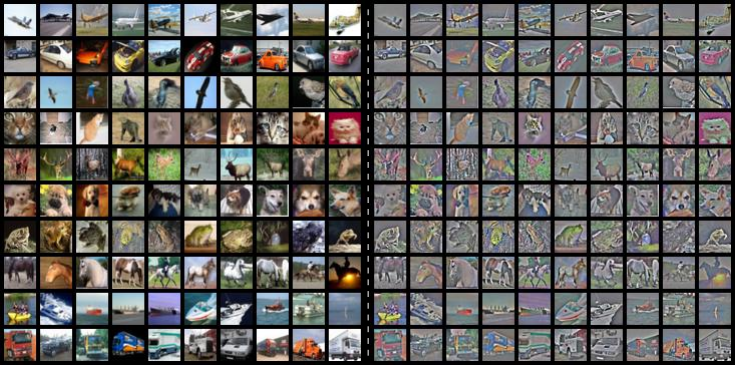
\includegraphics[width=14cm]{gambar/contoh_zca.png}
    \caption[Contoh-Contoh Hasil \acrshort{zca}]{Contoh-Contoh Hasil \acrshort{zca} \protect\shortcite{pal2016preprocessing}}
    \label{fig:contohhasilzca}
\end{figure}

\begin{figure}[t]
    \centering
    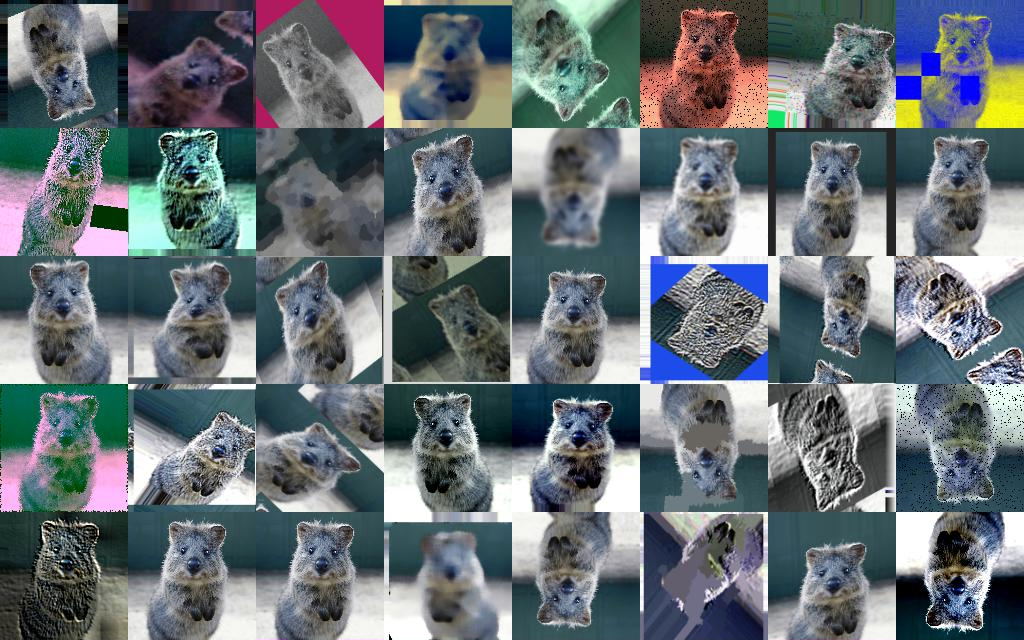
\includegraphics[width=14cm]{gambar/contoh_hasil_imgaug.png}
    \caption[Contoh-Contoh Hasil Augmentasi Data]{Contoh-Contoh Hasil Augmentasi Data (https://github.com/aleju/imgaug)}
    \label{fig:contohhasilimgaug}
\end{figure}

\begin{figure}[t]
    \centering
    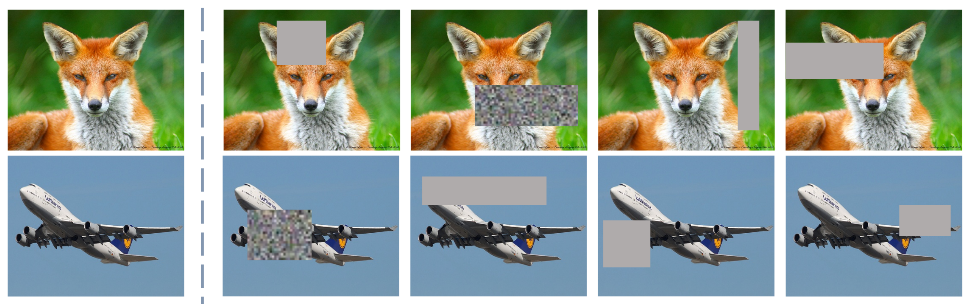
\includegraphics[width=14cm]{gambar/contoh_hasil_random_erasing.png}
    \caption[Contoh-Contoh Hasil Random Erasing]{Contoh-Contoh Hasil Random Erasing \protect\shortcite{zhong2017random}}
    \label{fig:contohrandomerasing}
\end{figure}

\textit{Data augmentation} biasa diterapkan untuk mengatasi \textit{overfitting} pada pelatihan model \acrshort{cnn} dengan set data yang terbatas. \textit{Data augmentation} dapat dilakukan baik menggunakan pendekatan konvensional (filter kernel, transformasi geometri, penghapusan acak, transformasi ruang warna dan pembauran gambar-gambar) maupun \textit{deep learning} (\textit{adversarial learning}, \textit{neural style transfer} dan GAN \textit{data augmentation}). \textit{Data augmentation} juga dapat dilakukan menggunakan \textit{meta learning}, yaitu paduan dari kedua pendekatan tersebut. Gambar \ref{fig:contohhasilimgaug} menunjukkan beberapa contoh hasil augmentasi data. Sejauh ini berdasarkan hasil eksperimen, pendekatan tradisional yang paling efektif dalam meningkatkan akurasi model adalah teknik \textit{cropping}, yaitu sebuah teknik pemrosesan gambar yang bekerja dengan menghilangkan sekumpulan piksel tertentu dari gambar \shortcite{shorten2019survey}. Di antara teknik \textit{cropping} yang paling populer dalam meningkatkan ketahanan model \acrshort{cnn} terhadap set data kecil adalah \textit{random erasing}, di mana teknik ini menghilangkan satu atau dua area piksel gambar secara acak (Gambar \ref{fig:contohrandomerasing}). Area-area gambar yang dihapus digantikan oleh piksel-piksel yang serupa atau sebarang \shortcite{zhong2017random,o2019comparing}. Penjelasan mendetail mengenai \textit{data augmentation} dapat dipelajari pada \shortciteA{shorten2019survey}.

\subsection{\textit{\acrlong{gcns}}}
\begin{figure}
    \centering
    \begin{subfigure}[t]{6.5cm}
        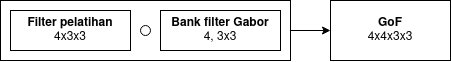
\includegraphics[width=6.5cm]{gambar/modulasi_gofs.png}
        \caption{Proses Modulasi \acrshort{gofs}}
        \label{fig:modulasigabor}
    \end{subfigure}
    ~~~
    \begin{subfigure}[t]{6.5cm}
        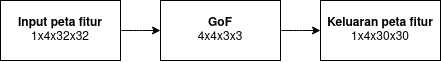
\includegraphics[width=6.5cm]{gambar/konvolusi_gofs.png}
        \caption{Contoh Konvolusi oleh \acrshort{gofs}}
        \label{fig:konvolusigofs}
    \end{subfigure}
    \caption[Modulasi dan Konvolusi \acrshort{gofs} di \acrshort{gcns}]{Modulasi dan Konvolusi \acrshort{gofs} di \acrshort{gcns} \protect\shortcite{luan2018gabor}}
    \label{fig:gofs}
\end{figure}
\begin{figure}[t]
    \centering
    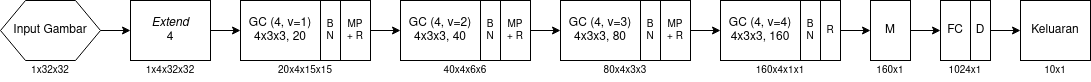
\includegraphics[width=14cm]{gambar/gcns.png}
    \caption*{\footnotesize{C---Konvolusi Spasial; MP---Max-Pooling; R---ReLu; M---Max; BN---BatchNormalization; D: Dropout}}
    \caption[Arsitektur \acrshort{gcns}]{Arsitektur \acrshort{gcns} \protect\shortcite{luan2018gabor}}
    \label{fig:gcns}
\end{figure}
\textit{\acrlong{gcns}} (\acrshort{gcns}), yang pertama kali diperkenalkan oleh \shortciteA{luan2018gabor}, merupakan \acrshort{dcnns} yang dimasuki oleh filter konvolusi \textit{\acrlong{gofs}} (\acrshort{gofs}) untuk meningkatkan ketahanan fitur yang dipelajari dalam perubahan skala dan orientasi. \acrshort{gofs} merupakan lapisan konvolusi dari modulasi filter pelatihan oleh filter Gabor dengan variasi skala dan orientasi. Gambar \ref{fig:gofs} menunjukkan bagaimana proses modulasi \acrshort{gofs} berlangsung. Sedangkan Gambar \ref{fig:gcns} menunjukkan bagaimana \acrshort{gofs} menempati setiap lapisan konvolusi pada jaringan tersebut.

\section{\textit{\acrlong{frs}}}
Pada studi segmentasi bagian wajah dalam konteks pengenalan ekspresi, tidak ada kesepakatan tentang bagaimana segmentasi yang optimal itu. Namun berdasarkan studi literatur, penulis menyimpulkan bahwa mayoritas penelitian menggunakan tiga bagian wajah yang paling menonjol pada pengenalan emosi. Ketiga bagian tersebut secara berurutan adalah mata, hidung, dan mulut \shortcite{guo2012holistic}. Proporsi kontribusi ketiga bagian tersebut hampir sama untuk setiap emosi \textit{angry}, \textit{disgust}, \textit{fear}, \textit{happy}, \textit{sad}, \textit{surprise}, dan \textit{neutral}. \shortciteA{benitez2018multicultural} membuktikan bahwa pengenalan ekspresi dengan tiga bagian ini mengungguli pengenalan menggunakan empat bagian, yaitu mata, hidung, mulut, dan dahi.

Segmentasi bagian wajah dapat dilakukan melalui berbagai cara, di antaranya melalui pendekatan \textit{grid/block based} dan \textit{local region based}. Dalam penelitian tersebut, mereka membagi wajah menjadi delapan belas bagian (Gambar \ref{fig:segmentasi18}) di mana area mata dibagi menjadi enam bagian, area hidung dibagi menjadi dua bagian dan sepuluh bagian sisanya untuk dahi, pipi dan dagu. Segmentasi area mulut pun dibuat sangat spesifik dengan membaginya berdasarkan garis luar bibir. Hasil eksperimen menunjukkan bahwa representasi \textit{local region based} lebih baik daripada representasi holistik dalam \textit{face registration} \shortcite{ghimire2015facial}. Ini menunjukkan bahwa mendefinisikan \acrshort{roi} secara spesifik dapat meningkatkan kualitas ekstraksi fitur.

% TODO: pustaka opencv (scaling, histogram equalization), FAN/RetinaFace (face detection + facial landmark detection), LogGabor dll.
